\documentclass{ueacmpstyle}


\RequirePackage{natbib}
\usepackage{graphicx}
\usepackage{caption}
\usepackage{appendix}
\usepackage[hyphens]{url}
\usepackage{float}
\usepackage{siunitx}
\graphicspath{/Images/}


\title{SARCA: A Conceptual Framework for Search and Rescue Canine Aided Operations} 
\author{
	Student ID: 100339217 and 100203834 \\
	Module: CMP7040B Ubiquitous Computing \\
	Word Count: 3740 (excluding references and appendix)
}
\date{\today}


\begin{document}

    \maketitle

    \section{Individual Contribution} \label{Sec: Individual Contribution}
        100203835: 50\%\\
        100339217: 50\%\\
        The group for this project comprised of two students, both of whom contributed evenly to the project either collectively on elements such as design and planning, or concurrently on elements such as development and testing.  Whilst not ideal, work was divided and handled in response to the global pandemic limiting the ability for the group members to meet or share resources.  Both members were involved in the early stages of the design process including the generation of ideas and identification of requirements. 100203834 then progressed researching and sourcing hardware components whilst 100339217 gave consideration to the User Interface (UI) design.  In a similar fashion, the decision was made for 100203834 to be in possession of the hardware and focus on creating the device and thereafter gathering and processing data.  100339217 did not have access to the hardware and therefore focused on supporting software, such as the android application, to receive and display the data to the user and provide functionality for connecting to the device. Where possible each member overlapped into the other area to share ideas and help out.  

    \section{Introduction}\label{Sec: Intro}
    The aim of this paper is to introduce a novel system that enables Search and Rescue (SAR) teams to augment and therefore alleviate the need for human interaction, when performing SAR operations. By developing a conceptual application that attempts to bridge the gap between previously developed Canine Augmented Technologies (CAT) and their respective canine's and handlers. Introducing SARCA (Search and Rescue Canine Aid, \textit{pronounced: sar-kah}), this report attempts to elaborate on a new conceptual framework for how CATs can be used within both SAR and USAR (Urban Search and Rescue) missions. The main objectives of this paper are to explain the SARCA framework, and provide a fundamental insight into the potential of this application. However, as there are limitations to the project - these will be discussed - the framework remains conceptual. This paper therefore attempts to explain the aims and motivations for the project, offer an insight into the features and spatial application of the SARCA device and the respective sensors and application.
    
    \subsection{Search and Rescue}
    Archetypally, there are two general avenues for SAR operations. Firstly, manned SAR operations - these are generally led on foot, and can be extremely dangerous; and secondly, unmanned SAR operations - these implement new technologies such as Unmanned Aerial Vehicles (UAVs) and animal-assisted SAR operations. However, both of these are not without their limitations. Manned SAR missions, typically start with by sending out a search party, to attempt to look for the missing person(s). Followed by manned aerial searches such as Helicopters. This raises two initial factors: They are time consuming, can be detrimental to health \citep{McRae2019} and are expensive \citep{Shakhatreh2019}. 
    
    \subsection{Canine Assist Technologies}
    Despite the aforementioned advances in SAR technology. The use of UAVs is limited to aerial application. Thus, if a missing person is located under rubble, for instance in a collapsed building due to an earthquake, or in a collapsed cave, their application is void. However, the implementation of canine-assisted SAR operations is too a developing field. There is limited research in the field, with research highlighting peer-to-peer communication of the handler and canine, and the use of wireless cameras attached to the canine's head \citep{Ferworn2006}. The previous works of \cite{Ferworn2006} are influential for the current report. They highlight that in many scenarios, the most effective methods of finding survivors is through the use of trained canine units. \cite{Ferworn2006} promote the implementation of CAT extensively. Specifying the use of audio and video communication, and GPS location. However, this leads to limitations when there is little to no light. Of which is common for SAR disasters \citep{Statheropoulos2014}, especially those in an urban setting. Alternatively, the works of \cite{Bozkurt2014} adopts a far more comprehensive array of sensors, with focus on the physiological attenuation of the canine whilst on a SAR operation. In lieu of both the \cite{Ferworn2006} and \cite{Bozkurt2014} reports, the current paper aims to develop a new conceptual model, targeted at SAR operations, with the fundamental concepts of CAT. 
    
    The current paper proposes the Search and Rescue Canine Aid (SARCA) framework, a completely modular CAT that implements a total of 14 sensory readings across 9 sensors. With each sensor providing a key insight into the environment and location of the area the canine is searching. A detailed list of the modules and their respective sensors can be found in section \ref{Sec: Sensing}. The conceptual model for the SARCA framework is presented in Fig. \ref{fig:conceptual}.
    
    \begin{figure}
        \begin{center}
            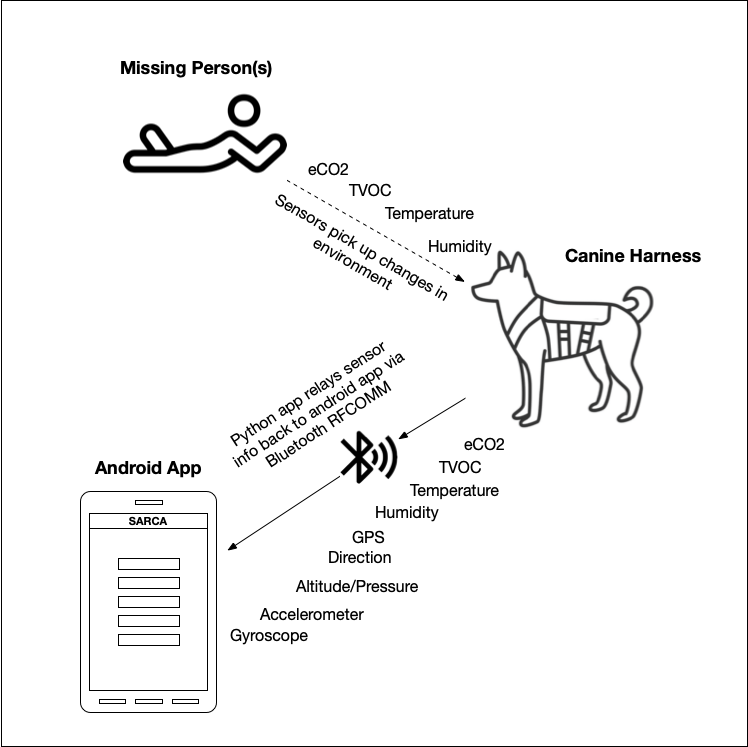
\includegraphics[scale=0.4]{Images/conceptualview.png}
            \caption{The SARCA Conceptual Framework}
            \label{fig:conceptual}
        \end{center}
    \end{figure}
    

        This paper aims to establish a conceptual framework with potential in-field application. The SARCA should be able to reliably monitor the environment in which it is surrounded, regardless of the condition or location. Moreover, the aim of the project is to establish a fundamental baseline of an empty room, over the period of 30 seconds. Following this, new thresholds will be applied to the model to determine that if a person is present in a room, how much the data varies from the baseline. Finally, if there is more than one person present, how much the data varies also. Using this data, it is possible to apply thresholds to the Android Application. Of which, acts as a probability indicator of likelihood of a survivor found. 
    
    \section{Sensing} \label{Sec: Sensing}
        This section aims to describe the reasoning behind the choices that were made for the development of this project. Specifically, elaborating on the rationale of why the following specific platforms were chosen and why others were not chosen.
        \subsection{Chosen Applications}
        
            \subsubsection{Raspberry Pi}
            The decision was made to use Raspberry Pi (RPi) model 4b 8GB, specifically due to the comprehensive list of ubiquitous computing accessories that can be added to it. Moreover, the RPi has a low-cost, especially for it's capabilities. The main contributing factor for choosing the Raspberry Pi, over anything else is it's built-in Bluetooth module. Therefore, minimising the cost of development of having to purchase an additional Bluetooth module. In addition to this, due to the large number of sensors that are being powered by the Raspberry Pi, the increased computing power of the 64 bit ARM processor, and the increased RAM size, offers unparalleled performance when compared to other miniature computers in the same class. 
            
            Furthermore, as most of the components in this project are modular, and easily removed. The RPi served as the building blocks for future development. Both the RPi and the Python code that runs the sensors, are modular. If and when necessary, more sensors can be added easily. Either by connecting the sensor to a new GPIO pin, or connecting it in series to a GPIO pin that is already in use and then the data can be accessed by adding the required files to the main Python program.  
            
            \subsubsection{DHT22}
            The DHT22\footnotemark[1] Humiture sensor was chosen to perform the Humidity and Temperature readings due to the extremely low cost per module, and low-error readings. The sensor can be powered from either a 3v or 5v input (essential for maintaining low-energy consumption); and is able to update the output once every two seconds. Moreover, it is able to capture humidity readings of 0 to 100\% with an accuracy of $\pm 5\%$ and temperature readings from -40$^\circ$C to 80$^\circ$C with an accuracy of $\pm 2^\circ$C per reading. Of course, these temperatures are unlikely in the simulated testing environment. However, they represent the type of robustness that would be needed in the field.
            \footnotetext[1]{Adafruit DHT22 Sensor -  {https://learn.adafruit.com/dht}}
        
            
            \subsubsection{SGP30}
            The SGP30\footnotemark[2] Multi-Pixel Gas Sensor was chosen due to the simplicity of implementation to read and provide accurate eCO2 (Equivalent Calculated Carbon Dioxide) and TVOC (Total Volatile Organic Compounds) without the need to stretch the I2C clocks. Specifically, the sensor is able to read eCO2 concentration in the range of 400 to 60,000 ppm (parts per million) and TVOC readings within a range of 0 to 60,000 ppb (parts per billion). Whilst maintaining a combined accuracy of $\pm15\%$. This sensor enables the development team to accurately read and monitor levels of Carbon Dioxide output in the instant environment, and interpret it for thresholds. 
            \footnotetext[2]{SGP30 MoX Sensor - https://www.adafruit.com/product/3709}
            
            \subsubsection{BerryIMU-GPS v4}
            The BerryIMU\footnotemark[3] is perhaps the center-piece of this project. Boasting seven sensors that can each be monitored logged throughout the data collection, including GPS, Speedometer, Accelerometer, Gyroscope, Magnetometer, Barometric/Altitude and Temperature. We chose this module, after consideration due to the small form factor, and ability to attach directly to the RPi as a HAT (Hardware Attached on Top). Firstly, the implementation of the GPS module, allows for real-time tracking of where the device is located, this is mandatory for equipment in SAR operations. Moreover, the Accelerometer, Gyroscope and Barometer allow for tracking the positioning of the canine. Once calibrated, the end user would be able to determine whether the canine is increasing or decreasing in altitude, and whether the canine has fallen. Initially, we were going to leave out the magnetometer due to the lack of user-friendliness regarding headings. However, the development team implemented a user-friendly version of headings, presented in a trivial manner. The temperature sensor on the BerryIMU is used as an internal measurement of the temperature. Acting as a CPU core temperature monitor, rather than environmental. 
            
            \footnotetext[3]{BerryIMU-GPS v4 - https://ozzmaker.com/product/berrygps-imu/}
            
            
            \subsubsection{Android Phone}
            The choice to use an Android Device as the main hosting platform for the application was trivial. Apple Products, specifically the iPhone, utilises the BLE (Bluetooth Low Energy) protocol, and therefore cannot communicate with the RFCOMM channel on the RPi. An alternative to this would be using the External Accessories framework in Xcode. However, this specifically requires a licence from Apple to do so. Therefore, creating an Android application that communicates via RFCOMM was the only viable option for developing the SARCA project. 
        
        \subsection{Alternative Applications}
        Initially, the choice was made to implement a standalone NEO V6 \footnotemark[4] GPS module. However, the breadboard we utilised did not offer the additional space another standalone module would need. Therefore, the choice was made to make this sensor redundant, and implement the BerryIMU sensor instead. 
        
        It should be noted, that this project would be possible to develop on smaller devices such as an Arduino, Orange Pi Prime, Banana Pi M3, Rock64 and Asus Tinker Board (as well as many others). However, due to the lack of Native Bluetooth support, as well as much lower processing capabilities. The developing team decided to adopt the use of a RPi.
        
        \footnotetext[4]{NEO v6 - https://www.electroschematics.com/neo-6m-gps-module/}
    
    
    \section{Data Collection Section} \label{Sec: Data Collection}
        The hardware utilised for data collection includes a RPi 4b 8GB, powered by an 10000mAh battery pack to allow for remote functionality. With the addition of a breadboard attached to the 40 pin GPIO (General Purpose Input/Output) connector of the Raspberry Pi. The following sensors were mounted to the breadboard, with the exception of the BerryGPS-IMU, which was mounted to the top of the Raspberry Pi (see Appendix \ref{app:finishedproject} for an example).
        
        Some of the sensors, primarily the GPS, barometer and accelerometer modules were acquired individually. However, with the implementation of the BerryGPS-IMU Hat, it enabled the project team to incorporate a larger and wider array of sensors, into a smaller overall footprint. 
        
        Formerly, a script was written in Python to handle the data collection. The aim of this script was to communicate with each of the sensors, and provide real-time feedback on the information that is being read. This data is then stored locally on the RPi in a log. In addition, the data was sent over Bluetooth through a RFCOMM (Radio-Frequency Communication) channel. An Android application was then developed to allow the end-user to connect their (Android) device to the Raspberry Pi, and have the real-time data displayed to them in a user-friendly manner. 
        
        The main intention of this device is to be used in SAR operations, to enable the SAR team to find and locate potentially missing persons. However, due to the ongoing uncertainty of the COVID-19 virus, it was not possible to collect the data in a field scenario. Specifically, a scenario representative of a SAR operation such as the \cite{McRae2019} case study to conduct a complex high altitude SAR operation. For these reasons, it is concluded that the data discussed hereon, is entirely simulated. Therefore, we base the findings entirely on the assumptions that can be drawn from the simulated data.
        
        In an attempt to be transparent, a top down view (with measurements and dimensions) has been provided in Appendix \ref{app:roomlayout}. The room utilises central heating, and has a radiator located under the window on the right of the \textit{X} (Width = 2 meters, Height = 40cm, Depth = 10cm). For the purpose of data collection, the central heating was switched off. However, the temperature outside was not measured. The results received therefore are likely to change dependant on this contributing factor. If the sensors exceeded this threshold, it would notify the user of the potential likelihood that a person has been located, along with the most recent data set.
        
    
    \section{Data Processing and Interpretation} \label{Sec: Data Processing}
        
        Due to the ongoing issues revolving around the COVID - 19 virus, it was not possible to reflect the findings in a manner representative of a real-world application. Therefore, it should be reiterated that all data presented in this report is simulated.
        
        \subsection{Descriptive Statistics}
        
        Each sensor was measured against the data from the respective baseline, for instance, all of the temperature data was compared against the base temperature. To protect against a Type 1 error, a Bonferroni correction was conducted in an attempt to reduce family-wise error. With the critical \textit{p} value adjusted to .0125 as the new threshold for significance. 
        
        The data was collected in five stages. Firstly, to establish a baseline over a period of time, the device was left in the room (see Appendix \ref{app:roomlayout} unattended as to not manipulate the values read by the sensor. This was then repeated for the other four conditions, respective of: One person more than one meter away from the device (m1m1p); One person less than one meter away from the device (l1m1p); two people more than one meter away (m1m2p) and finally, two people less than one meter away (l1m2p).
        
        The mean proportional sensor value was calculated for each set of sensors and the respective conditions is represented in Figure \ref{fig:MeanValues}. The baseline values for this comparison can be found in Appendix \ref{means}
        
        \begin{center}
            \begin{figure}
                \centering
                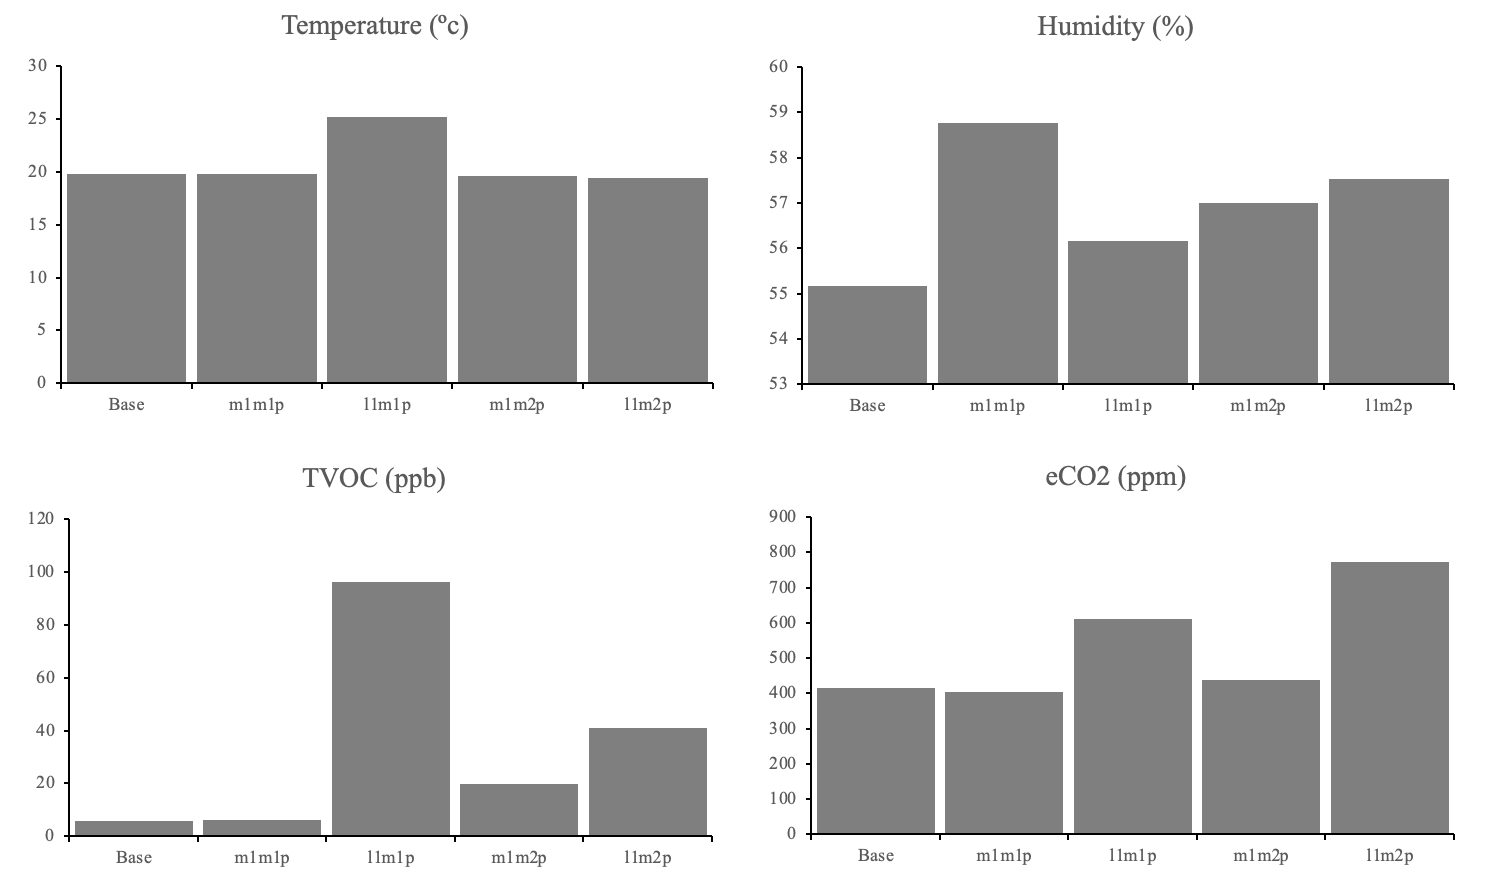
\includegraphics[scale=0.5]{Images/average.png}
                \caption{Mean values for each condition}
                \label{fig:MeanValues}
            \end{figure}
        \end{center}
        
        
        
        Following this, a simple linear regression was carried out on each of the conditions to investigate the relationship between temperature, humidity, eCO2 and TVOC and elapsed time (seconds). For temperature, the scatter plot (see \ref{App: }) show that there was a strong positive linear relationship between the two, which was confirmed with a Pearson's correlation coefficient of \textit{r} = .765. Similar linear regression showed a significant relationship between temperature and elapsed time (\textit{p} < .001). The slope coefficient for m1m1p was -.169, so the temperature decreases .169 degrees every second for each second of elapsed time. The slope coefficient for l1m1p was -.041, so the temperature decease .041 degrees every second for each second of elapsed time. The slope coefficient for m1m2p was .330, so the temperature increases .330 degrees for every second for each second of elapsed time. The slope coefficient for l1m2p was .137, so the temperature increases .137 degrees for every second of elapsed time. The \textit{R$^2$} value was 0.586 so 58.6\% of the variation in temperature can be explained by elapsed time. The scatter plot of standardised predicted values versus standardised residuals, showed that the data met the assumptions of homogeneity of variances and linearity and the residuals were approximately normally distributed. 

        
        For humidity, the scatter plot indicated that there was a positive linear relationship between the two, \textit{r} = .544. Simple linear regression showed mixed results, showing a significant result between humidity and elapsed time in the m1m2p and l1m2p conditions, both reporting \textit{p} < .001. Whereas in the conditions m1m1p and l1m1p there was no significant relationship to the control, \textit{p} = .25 and \textit{p} = .974 respectively. The slope coefficient for m1m1p was -.04, so the humidity decreases .04\% for every second of elapsed time. The slope coefficient for l1m1p was .0007, so the humidity increases .0007\% for every second of elapsed time. The slope coefficient for m1m2p was -.04, so the humidity increases .19\% for every second of elapsed time. The slope coefficient for l1m2p was -.04, so the humidity decreases .022\% for every second of elapsed time. The \textit{R$^2$} value was 0.544 so 54.4\% of the variation in humidity can be explained by elapsed time. The scatter plot of standardised predicted values versus standardised residuals, showed that the data violated the assumptions of homogeneity of variances and linearity and the residuals were approximately normally distributed. 

        
        For eCO2, there was a strong positive relationship between the two, \textit{r} = .908. Simple linear regression showed mixed results between eCO2 and elapsed time in the m1m1p, m1m2p and l1m2p conditions, reporting \textit{p} < .001, \textit{p} = .003 and \textit{p} < .001 respectively. However in the l1m1p condition there was no significant relationship to the control \textit{p} = .110. The slope coefficient for m1m1p was .146, so the eCO2 increases .146 ppm for every second of elapsed time. The slope coefficient for l1m1p was -.003, so the eCO2 decreases .003ppm for every second of elapsed time. The slope coefficient for m1m2p was .423, so the eCO2 increases .423ppm for every second of elapsed time. The slope coefficient for l1m2p was -.021, so the eCO2 decreases .021ppm for every second of elapsed time. The \textit{R$^2$} value was 0.824 so 82.4\% of the variation in eCO2 can be explained by elapsed time. The scatter plot of standardised predicted values versus standardised residuals, showed that the data met the assumptions of homogeneity of variances and linearity and the residuals were approximately normally distributed.
        
        For TVOC, there was a weak positive linear relationship between the two, which was confirmed as \textit{r} = .265. Simple linear regression showed there was a non significant relationship between TVOC and elapsed time \textit{p} = .04. The slope coefficient for m1m1p was .074, so the TVOC increases .74 ppb for every second of elapsed time. The slope coefficient for l1m1p was -.012, so the TVOC decreases .012 ppb for every second of elapsed time. The slope coefficient for m1m2p was .121, so the TVOC increases .121 ppb for every second of elapsed time. The slope coefficient for l1m2p was .020, so the TVOC increases .020 ppb for every second of elapsed time. The \textit{R$^2$} value was 0.7 so 70\% of the variation in TVOC can be explained by elapsed time. The scatter plot of standardised predicted values versus standardised residuals, showed that the data met the assumptions of homogeneity of variances and linearity and the residuals were approximately normally distributed. 
        
        
        
        
        
    
    \section{System Output and Feedback} \label{Sec: Output and Feedback}
        
        The nature of the product is that the sensor hardware would be attached to the SAR dogs harness, and would remotely report information from the sensors back to the handler or device user.  As such, on-board display devices were therefore discounted and it was accepted that some sort of display device would need to remain with the handler or user.  The decision was made early on that system output would be displayed to the user via a mobile application, and more specifically an android device as discussed in section \ref{Sec: Sensing}.  This also highlighted the requirement for the transmission of data wirelessly and potentially over reasonably long distances.  Due to the time and resource limitations of this project, it was agreed that at this stage a bluetooth connection would be used to establish communication between the android application and the harness device via RFCOM.  However, to extend the signal range, future research and development for this project would include investigation into the use of mobile data (4G or 5G connectivity) and radio controls.  The former would also incorporate consideration of hosting a web application as opposed to an android application, and allowing other users access during an active session.  For example, the session may be launched and managed on the ground by the SAR personnel utilising the mobile device, however further SAR colleagues may also be accessing from a desktop computer in a control room as they oversee the operation or coordinate the teams response.
        
        Initial Lo-Fi prototypes were produced, as seen in Appendix \ref{app:design} figures \ref{Figure Lofi v1 1} to \ref{Figure Lofi v1 6}.  Layout ideas were developed by the team to display summaries of the data collected, as well as more in depth analysis.  Aspirations to develop a full application were soon perceived to be unobtainable within the scope of this project and as such the application was scaled back to provide two key features; a means to successfully establish a bluetooth connection with the Raspberry Pi and the display of sensor data in a format beneficial and understandable to the user.  Version 2 of the Lo-Fi prototypes were produced, as included in Appendix \ref{app:design} figures \ref{Figure Lofi v2 1} and \ref{Figure Lofi v2} and these were utilised to build out the initial versions of the android application.  Screenshots of the application on an emulator are included in Appendix \ref{app:application}.  Figure \ref{Figure App before connection} shows the single page layout operating utilising a scroll view as shown in the prototypes.  Text views, list views and buttons are all dynamically added or removed depending on the users actions.  For example, it can be seen in figure \ref{Figure App Bonded} that once `Find Devices' has been clicked, a list view of devices in range and discoverable is populated.  Once a device is selected (via the onItemClickListener assigned to the items in the list view) the information at the top of the screen changes to show device connection and a `Get Connection` button has become available.  This improves usability by provided a more straightforward layout and disabling actions that the user may not be able to perform at that time.  Figure \ref{Figure App Send Message} shows the send message feature hosted within an Alert Dialog.  This enables the user to send a message from the android application to the Raspberry Pi.  At this stage, the relevant code has not been programmed into the python script to enable the Pi to handle this however the foundations have been laid and this would be an important future step to enable two way communication with the remote device.  
        
        Figure \ref{Figure App In Action} shows the SARCA android application in action with the remote device.  At this point the mobile device is connected to the Raspberry Pi and receiving information from the sensors which is in turn displayed as an `Incoming Message' on the phone screen.  This presents the latest information received from the device for all sensors however, the information is stored separately and historically in list variables within the android application.  The `Humiture Data' button which can be seen toward the bottom of the screen calls upon this stored information to display just humiture data so that the user can review changes over time or throughout the rescue operation. 
    
    \section{Conclusion} \label{Sec: Conclusion}
        \textit{This  section  should  give  a concluding  overview  of  the  whole  system.  It  should  summarize  the  systems merits and shortcomings in relation to any testing/evaluation that was done in each of the sections as well as in relation to the original aims and the real-world problem to be solved.This section should also refer to the systems and past works referred to in the Background section.}

    
    \bibliographystyle{apalike}
    \bibliography{FinalProject_bib}
    
    \newpage
    \section{Appendices}
    \appendix
        \section{Data Collection - Room Layout}\label{app:roomlayout}
        \begin{center}
            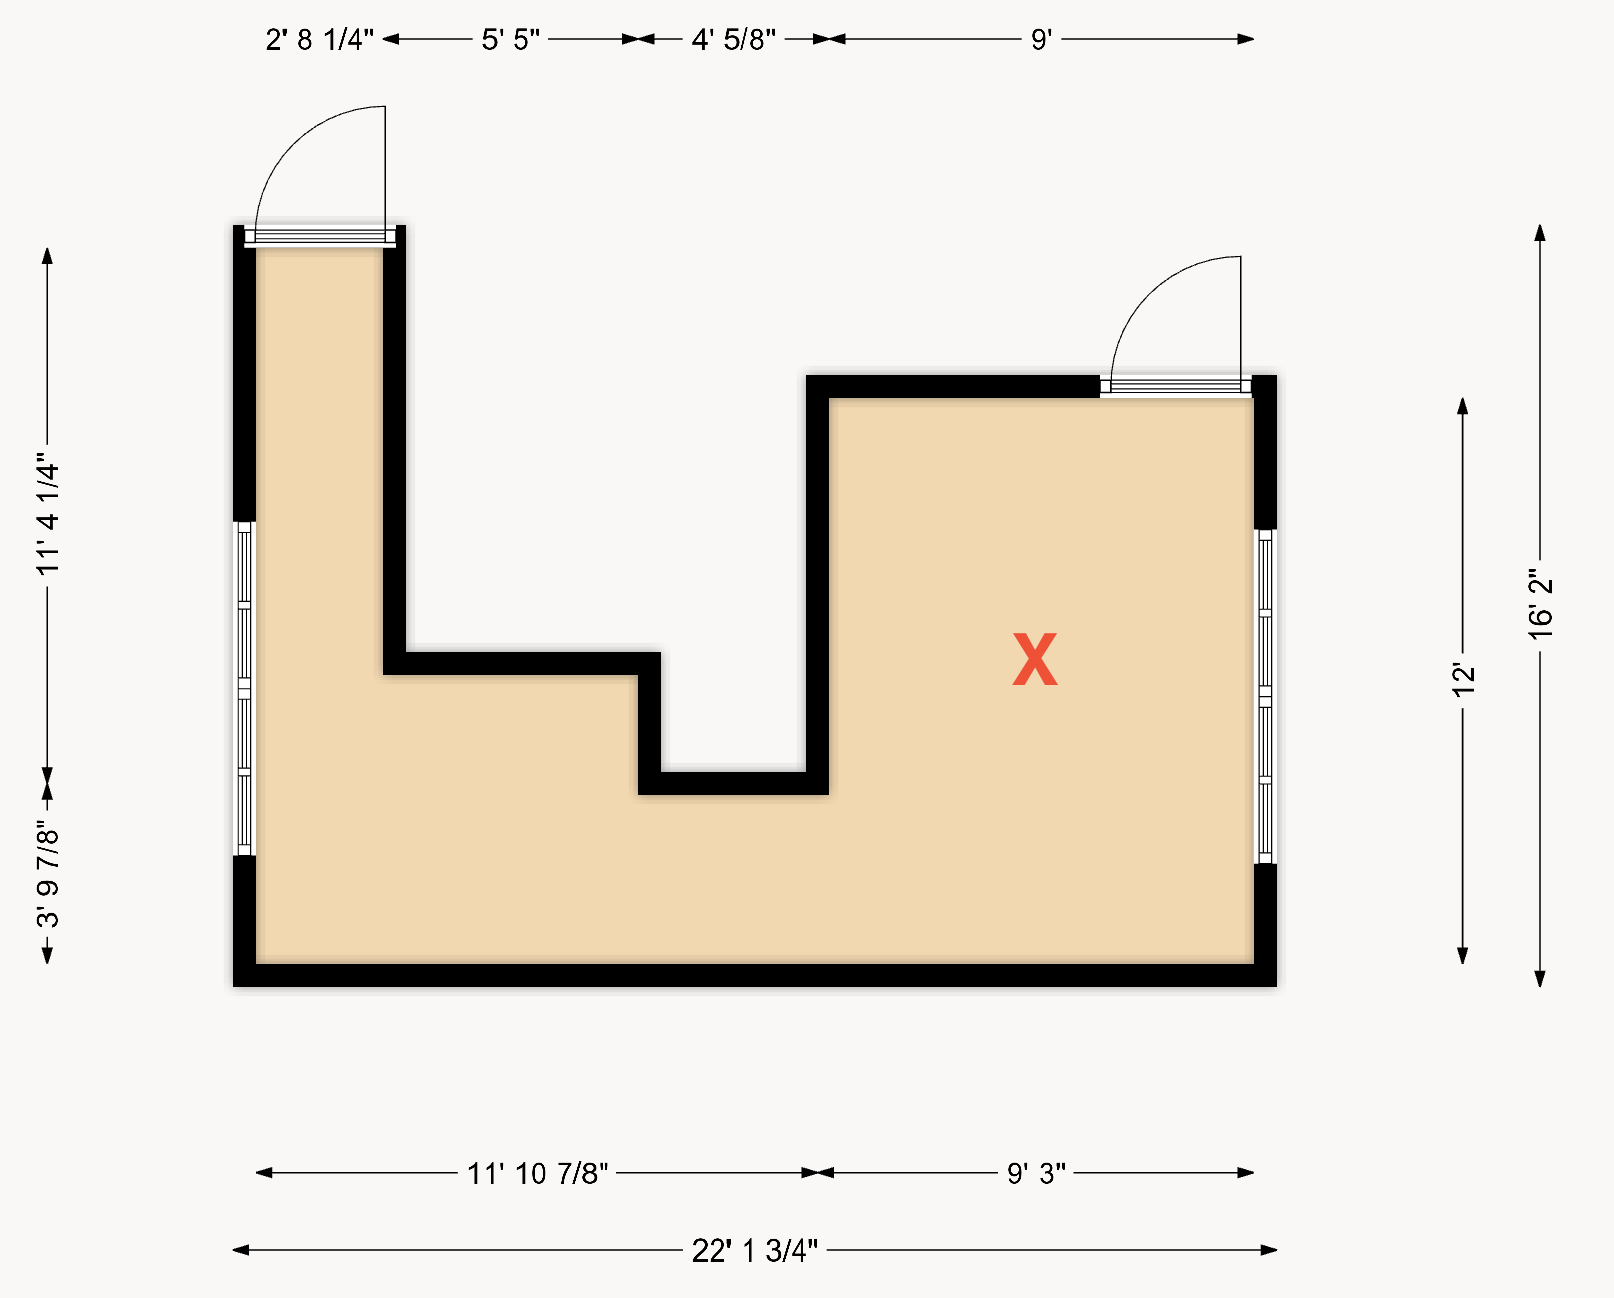
\includegraphics[scale=0.5]{Images/room.png}
        \end{center}
        A top down view of the room that the data was collected in. The \textit{X} represents where the SARCA device was situated throughout each condition. 
        
        \section{SARCA - Overview of setup}\label{app:finishedproject}
        
        \section{Scatter}
            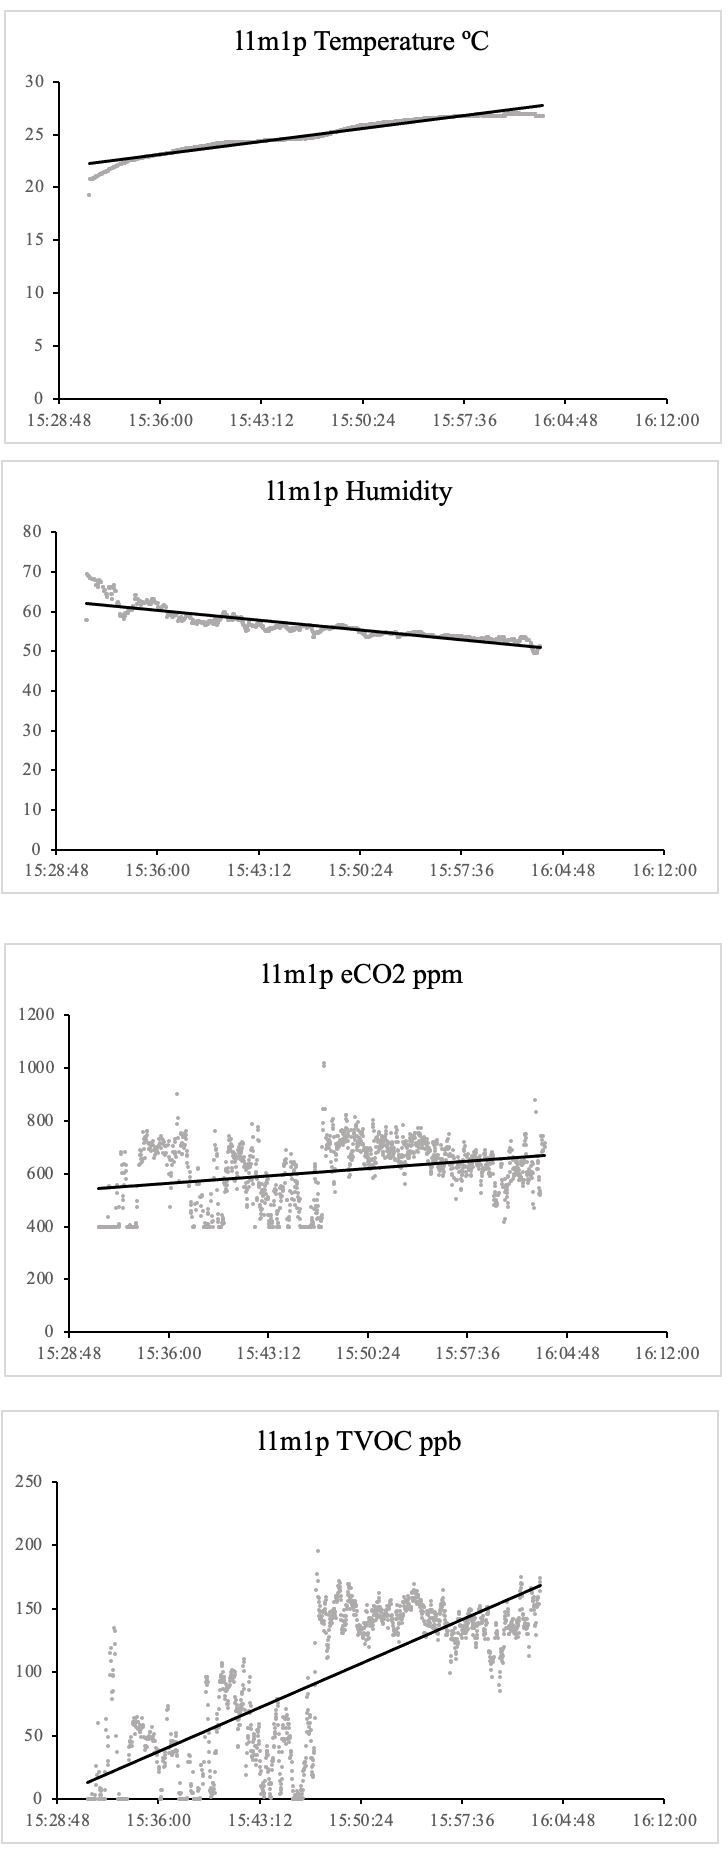
\includegraphics[scale=0.3]{Images/l1m1p.png}
            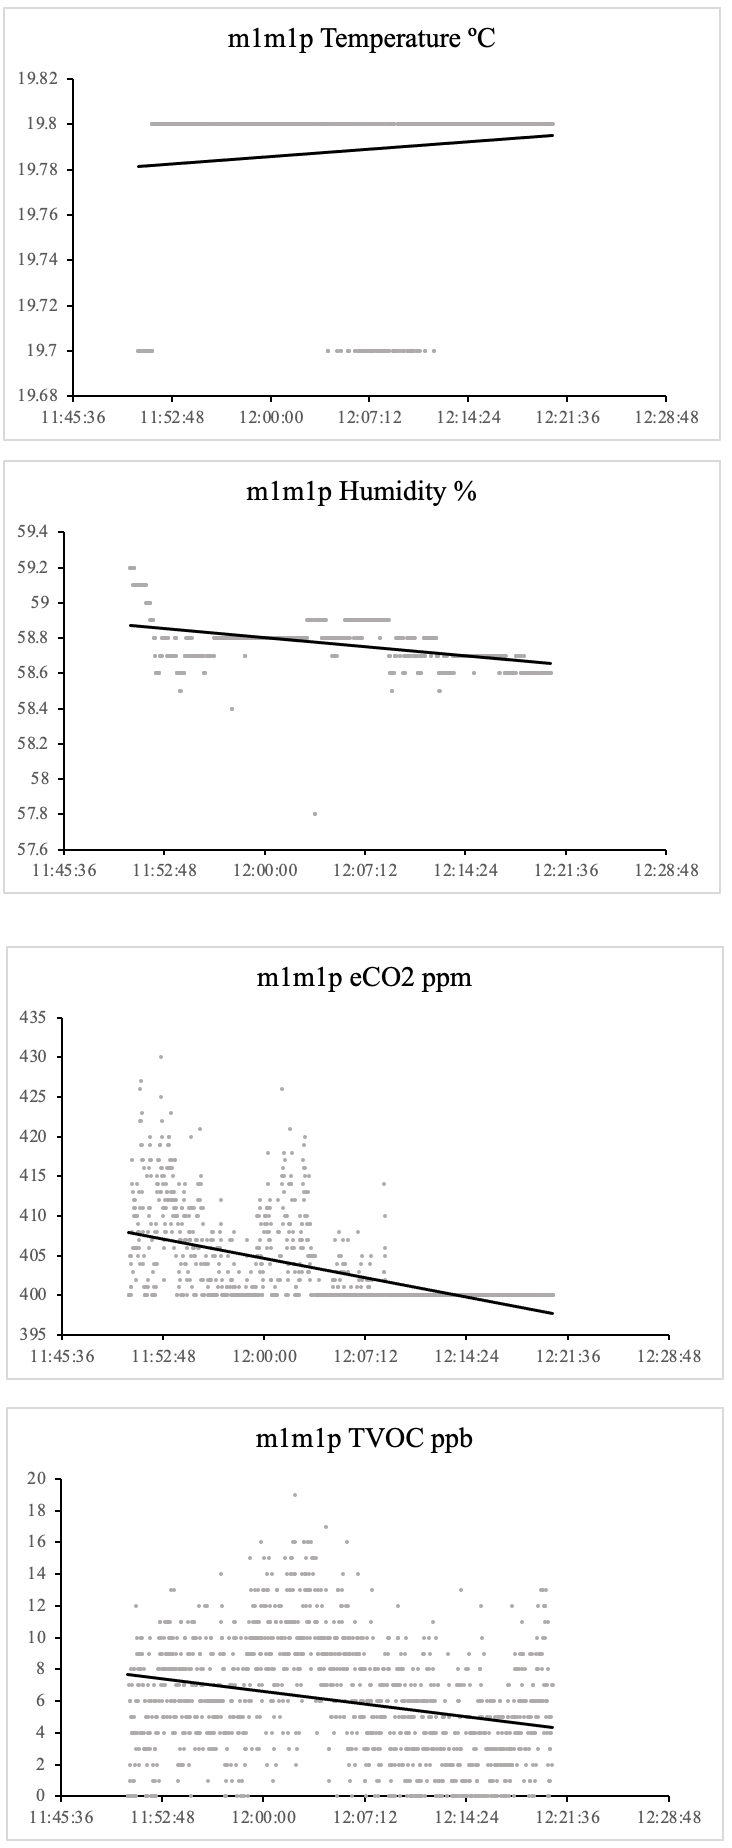
\includegraphics[scale=0.3]{Images/m1m1p.png}
            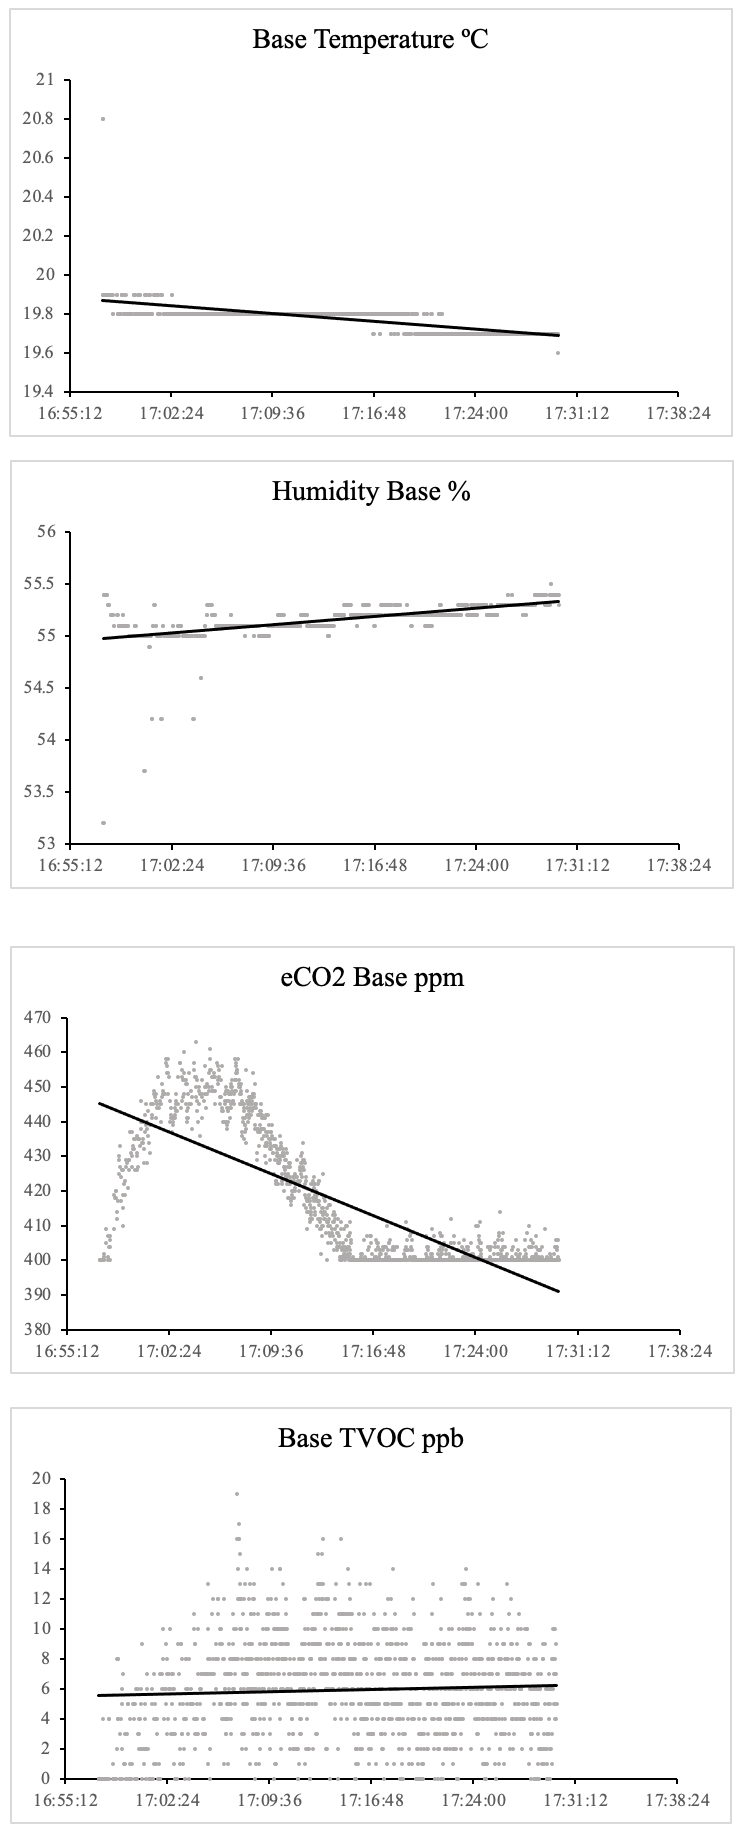
\includegraphics[scale=0.3]{Images/base.png}
            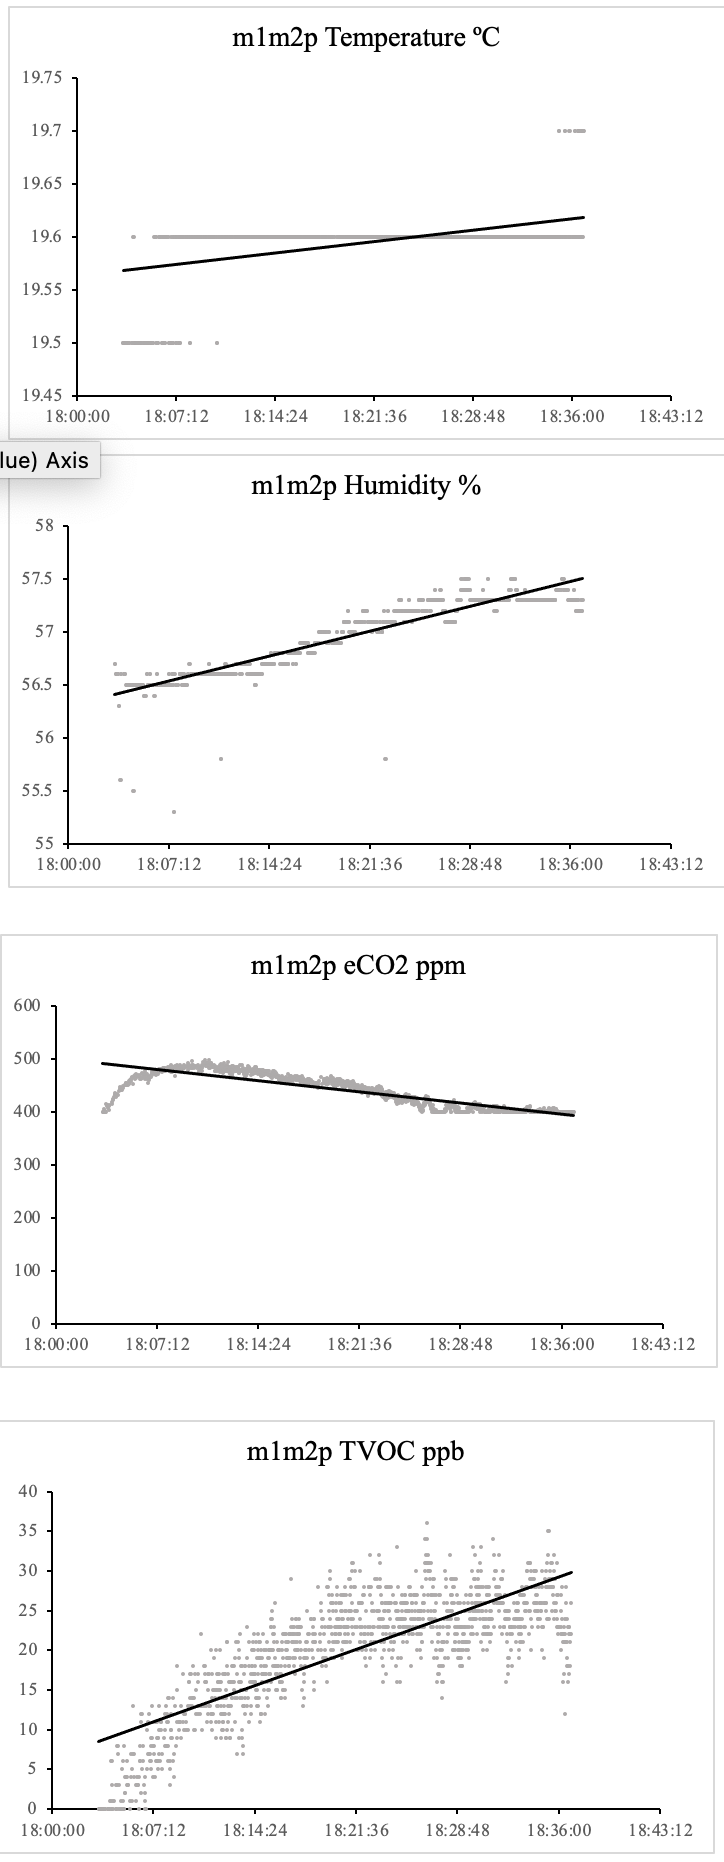
\includegraphics[scale=0.3]{Images/m1m2p.png}
            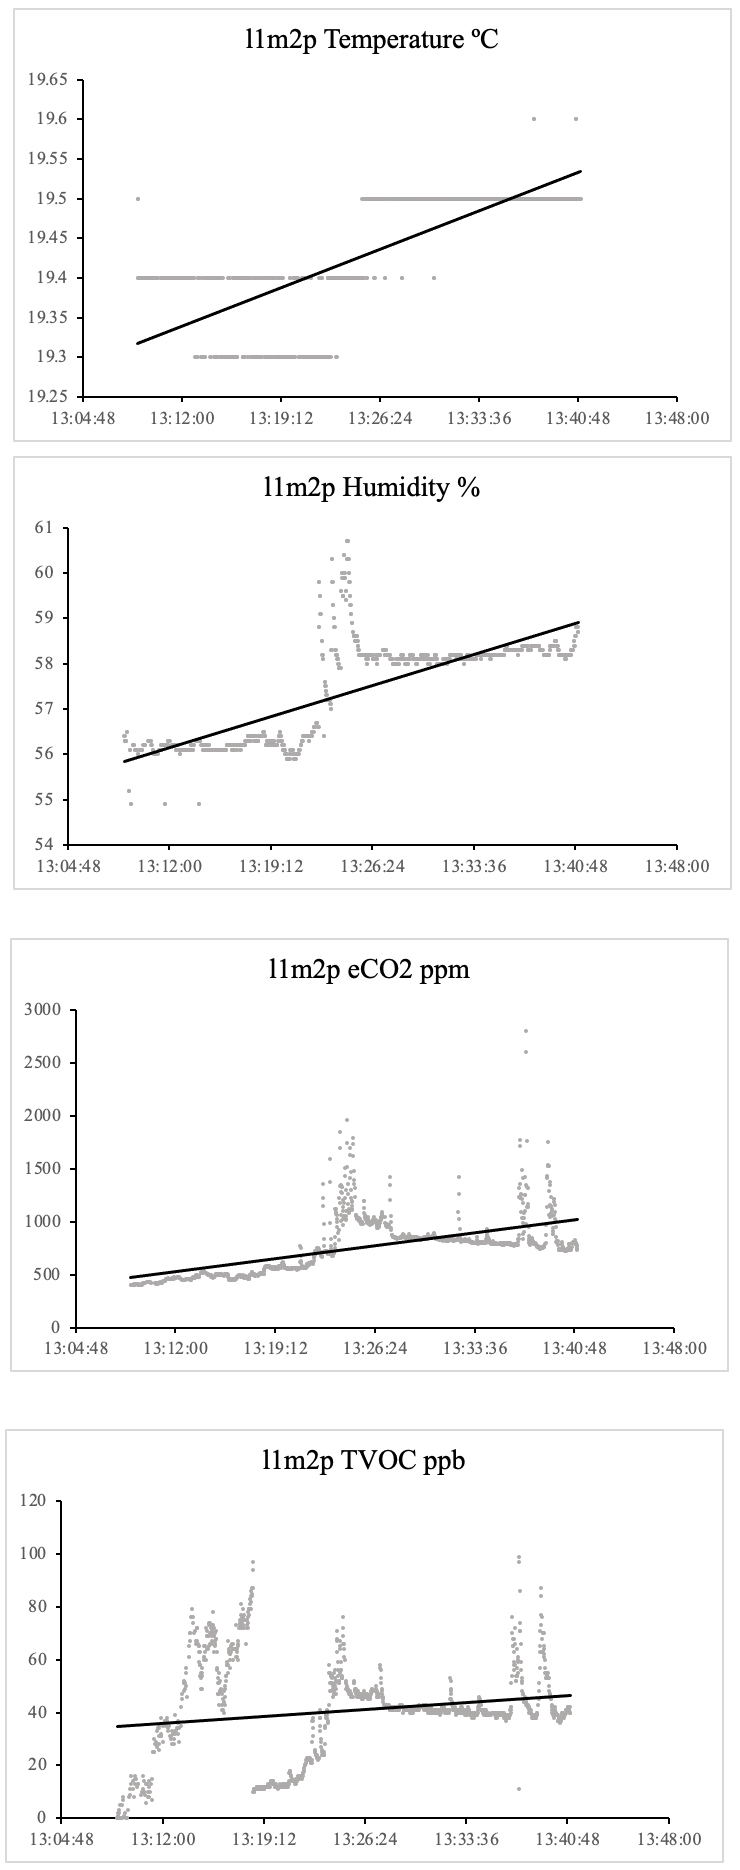
\includegraphics[scale=0.3]{Images/l1m2p.png}
        \newpage
        \section{Mean Analysis}\label{means}
        \textit{Baseline} Temperature: \textit{N} = 1343, \textit{M} = 19.77, (\textit{SE} = .001), \textit{SD} = .068, 95\% CI [19.766, 19.773]; Humidity: \textit{N} = 1343, \textit{M} = 55.17, (\textit{SE} = .004), \textit{SD} = .159, 95\% CI [55.1643, 55.1814]; eCO2: \textit{N} = 1343, \textit{M} - 415.5, (\textit{SE} = .51), \textit{SD} = 18.8, 95\% CI [414.4942, 416.5080]; TVOC: \textit{M} - 5.94, (\textit{SE} = .09), \textit{SD} = 3.43, 95\% CI [5.7575, 6.1248]. 
        
        \textit{M1m1p} Temperature: \textit{N} = 1343, \textit{M} = 19.79, (\textit{SE} = .001), \textit{SD} = .032, 95\% CI [19.7864, 19.7898]; Humidity: \textit{N} = 1343, \textit{M} = 58.77, (\textit{SE} = .004), \textit{SD} = 0.13, 95\% CI [58.758, 58.772]; eCO2: \textit{N} = 1343, \textit{M} = 402.1, (\textit{SE} = .14), \textit{SD} = 5.16, 95\% CI [402.624, 403.176]; TVOC: \textit{M} = 6.03, (\textit{SE} = .10), \textit{SD} = 3.76, 95\% CI [5.7575, 6.1248].
    
        \textit{L1m1p} Temperature: \textit{N} = 1343, \textit{M} = 25.17, (\textit{SE} = 0.04), \textit{SD} = 1.51, 95\% CI [25.09, 25.25]; Humidity: \textit{N} = 1343, \textit{M} = 56.17, (\textit{SE} = .09), \textit{SD} = .159, 95\% CI [55.99, 56.35]; eCO2: \textit{N} = 1343, \textit{M} = 612.1, (\textit{SE} = .3.08), \textit{SD} = 113, 95\% CI [606, 618]; TVOC: \textit{M} = 96.28, (\textit{SE} = 1.5), \textit{SD} = 55.25, 95\% CI [93.29, 99.2].
        
        \textit{M1m2p} Temperature: \textit{N} = 1343, \textit{M} = 19.6, (\textit{SE} < .001), \textit{SD} = .002, 95\% CI [19.593, 19.596]; Humidity: \textit{N} = 1343, \textit{M} = 56.9, (\textit{SE} = .009), \textit{SD} = .33, 95\% CI [56.98, 57.02]; eCO2: \textit{N} = 1343, \textit{M} = 438.8, (\textit{SE} = .86), \textit{SD} = 31, 95\% CI [437.10, 440.51]; TVOC: \textit{M} = 19.99, (\textit{SE} = 0.2), \textit{SD} = 7.39, 95\% CI [19.59, 20.38].
        
        \textit{L1m2p} Temperature: \textit{N} = 1343, \textit{M} = 19.45, (\textit{SE} = .002), \textit{SD} = .07, 95\% CI [19.431, 19.439]; Humidity: \textit{N} = 1343, \textit{M} = 57.52, (\textit{SE} = .02), \textit{SD} = 1.07, 95\% CI [57.46, 57.57]; eCO2: \textit{N} = 1343, \textit{M} = 771.95, (\textit{SE} = 7.07), \textit{SD} = 259.3, 95\% CI [758, 785]; TVOC: \textit{M} = 41.02, (\textit{SE} = 0.48), \textit{SD} = 17.5, 95\% CI [40.1, 41.9].
        
        
        \newpage
        \section{Design}\label{app:design}
            \subsection{Lo-Fi Prototypes Version 1}
            \begin{figure}[h]
                
                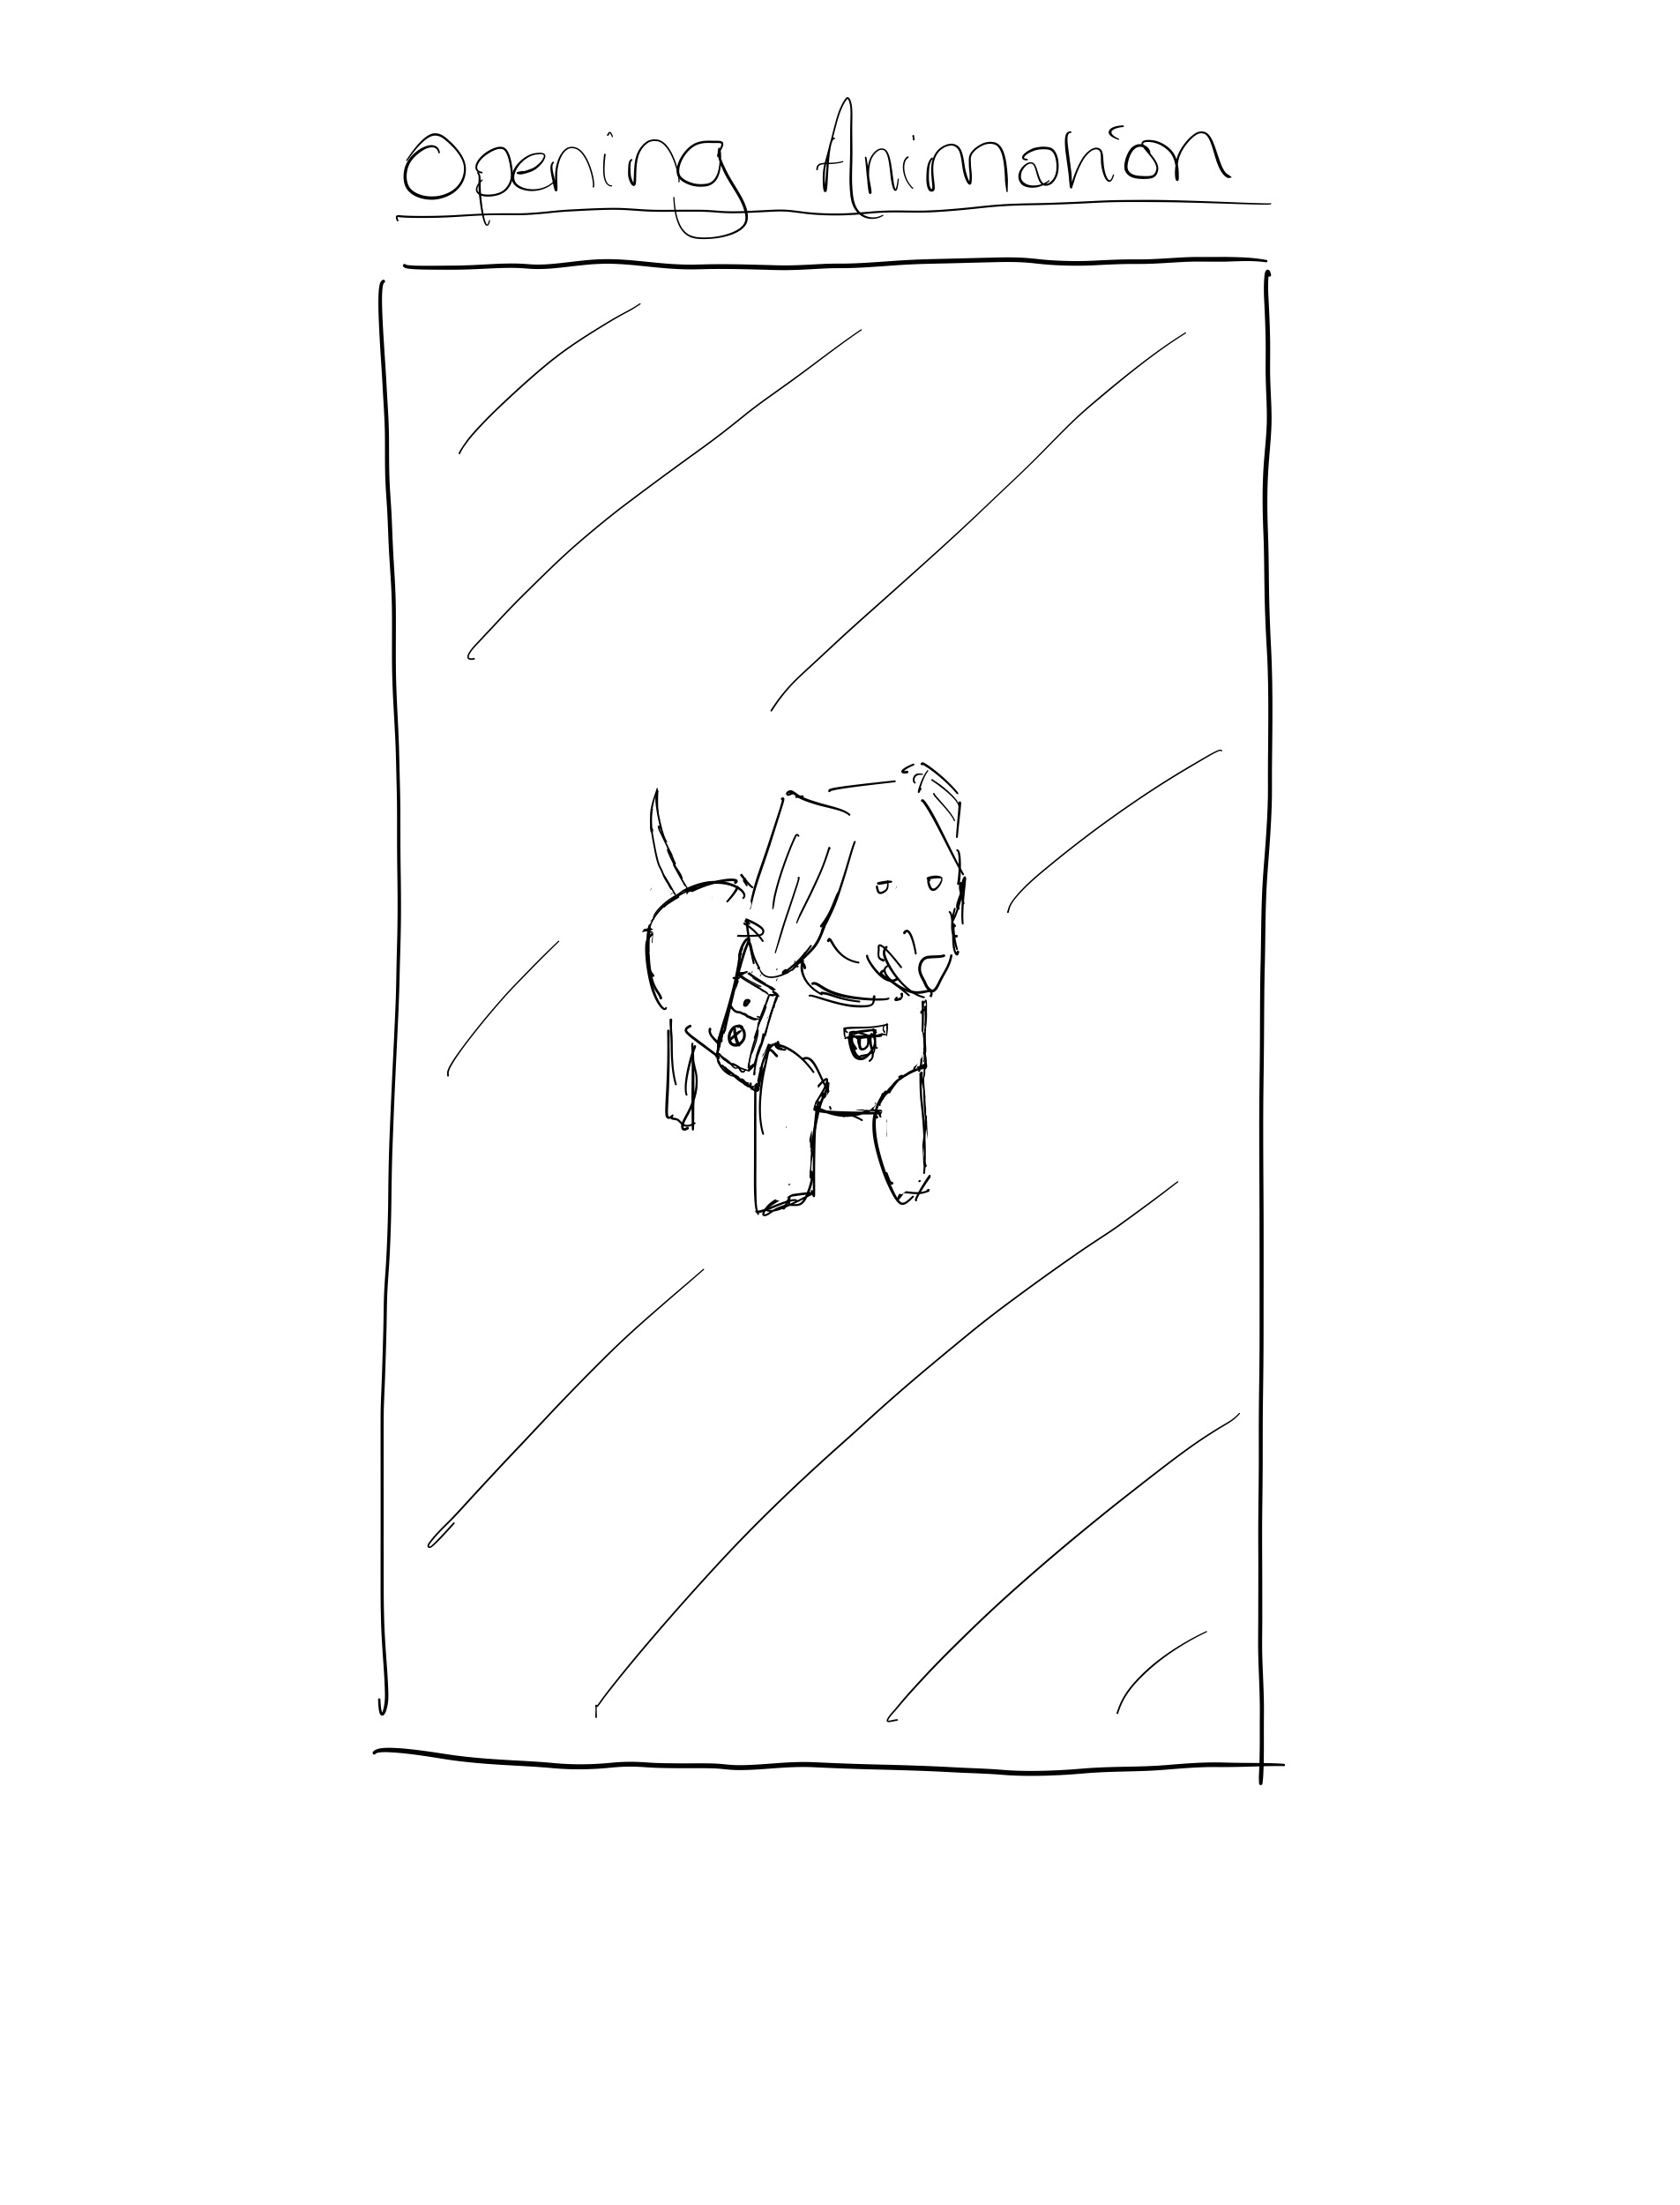
\includegraphics[width=\linewidth]{Images/Lofi_v1_a.jpg}
                \caption{Lo-Fi Prototype Version 1 Page 1}
                \label{Figure Lofi v1 1}
            
            \end{figure}
            \clearpage
            \begin{figure}[h]
                
                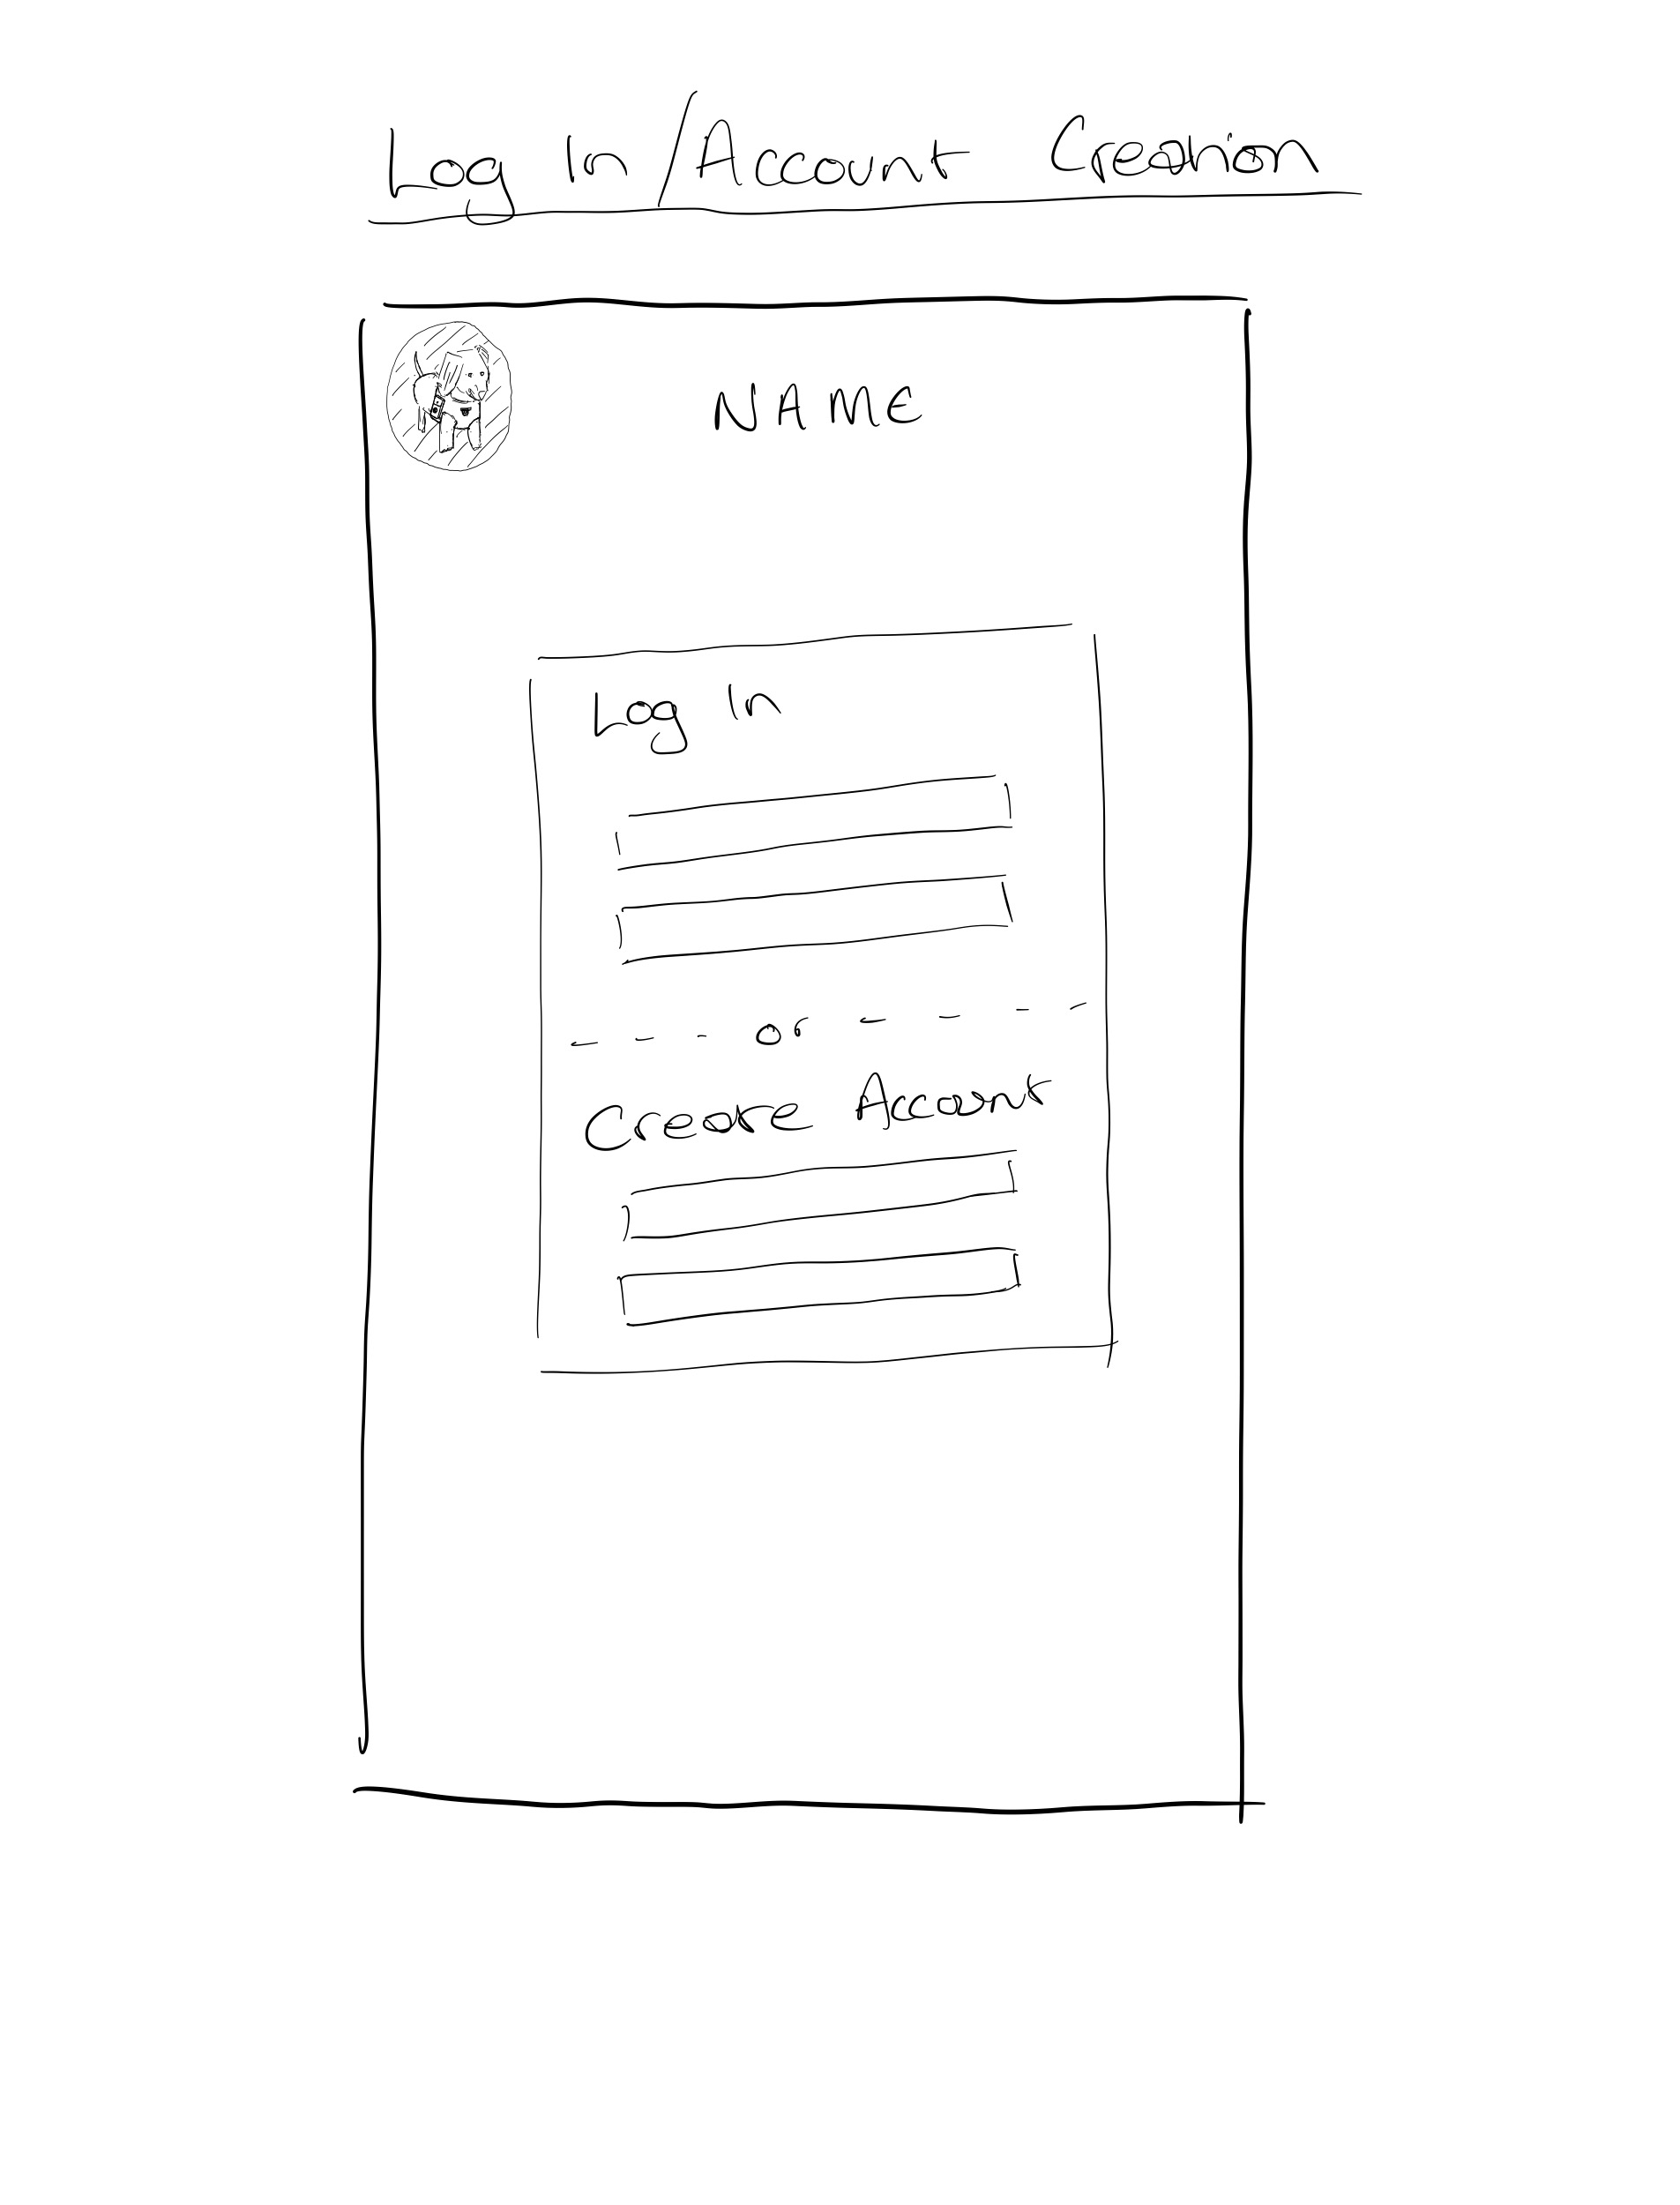
\includegraphics[width=\linewidth]{Images/Lofi_v1_b.jpg}
                \caption{Lo-Fi Prototype Version 1 Page 2}
                \label{Figure Lofi v1 2}
            
            \end{figure}
            \clearpage
            \begin{figure}[h]
                
                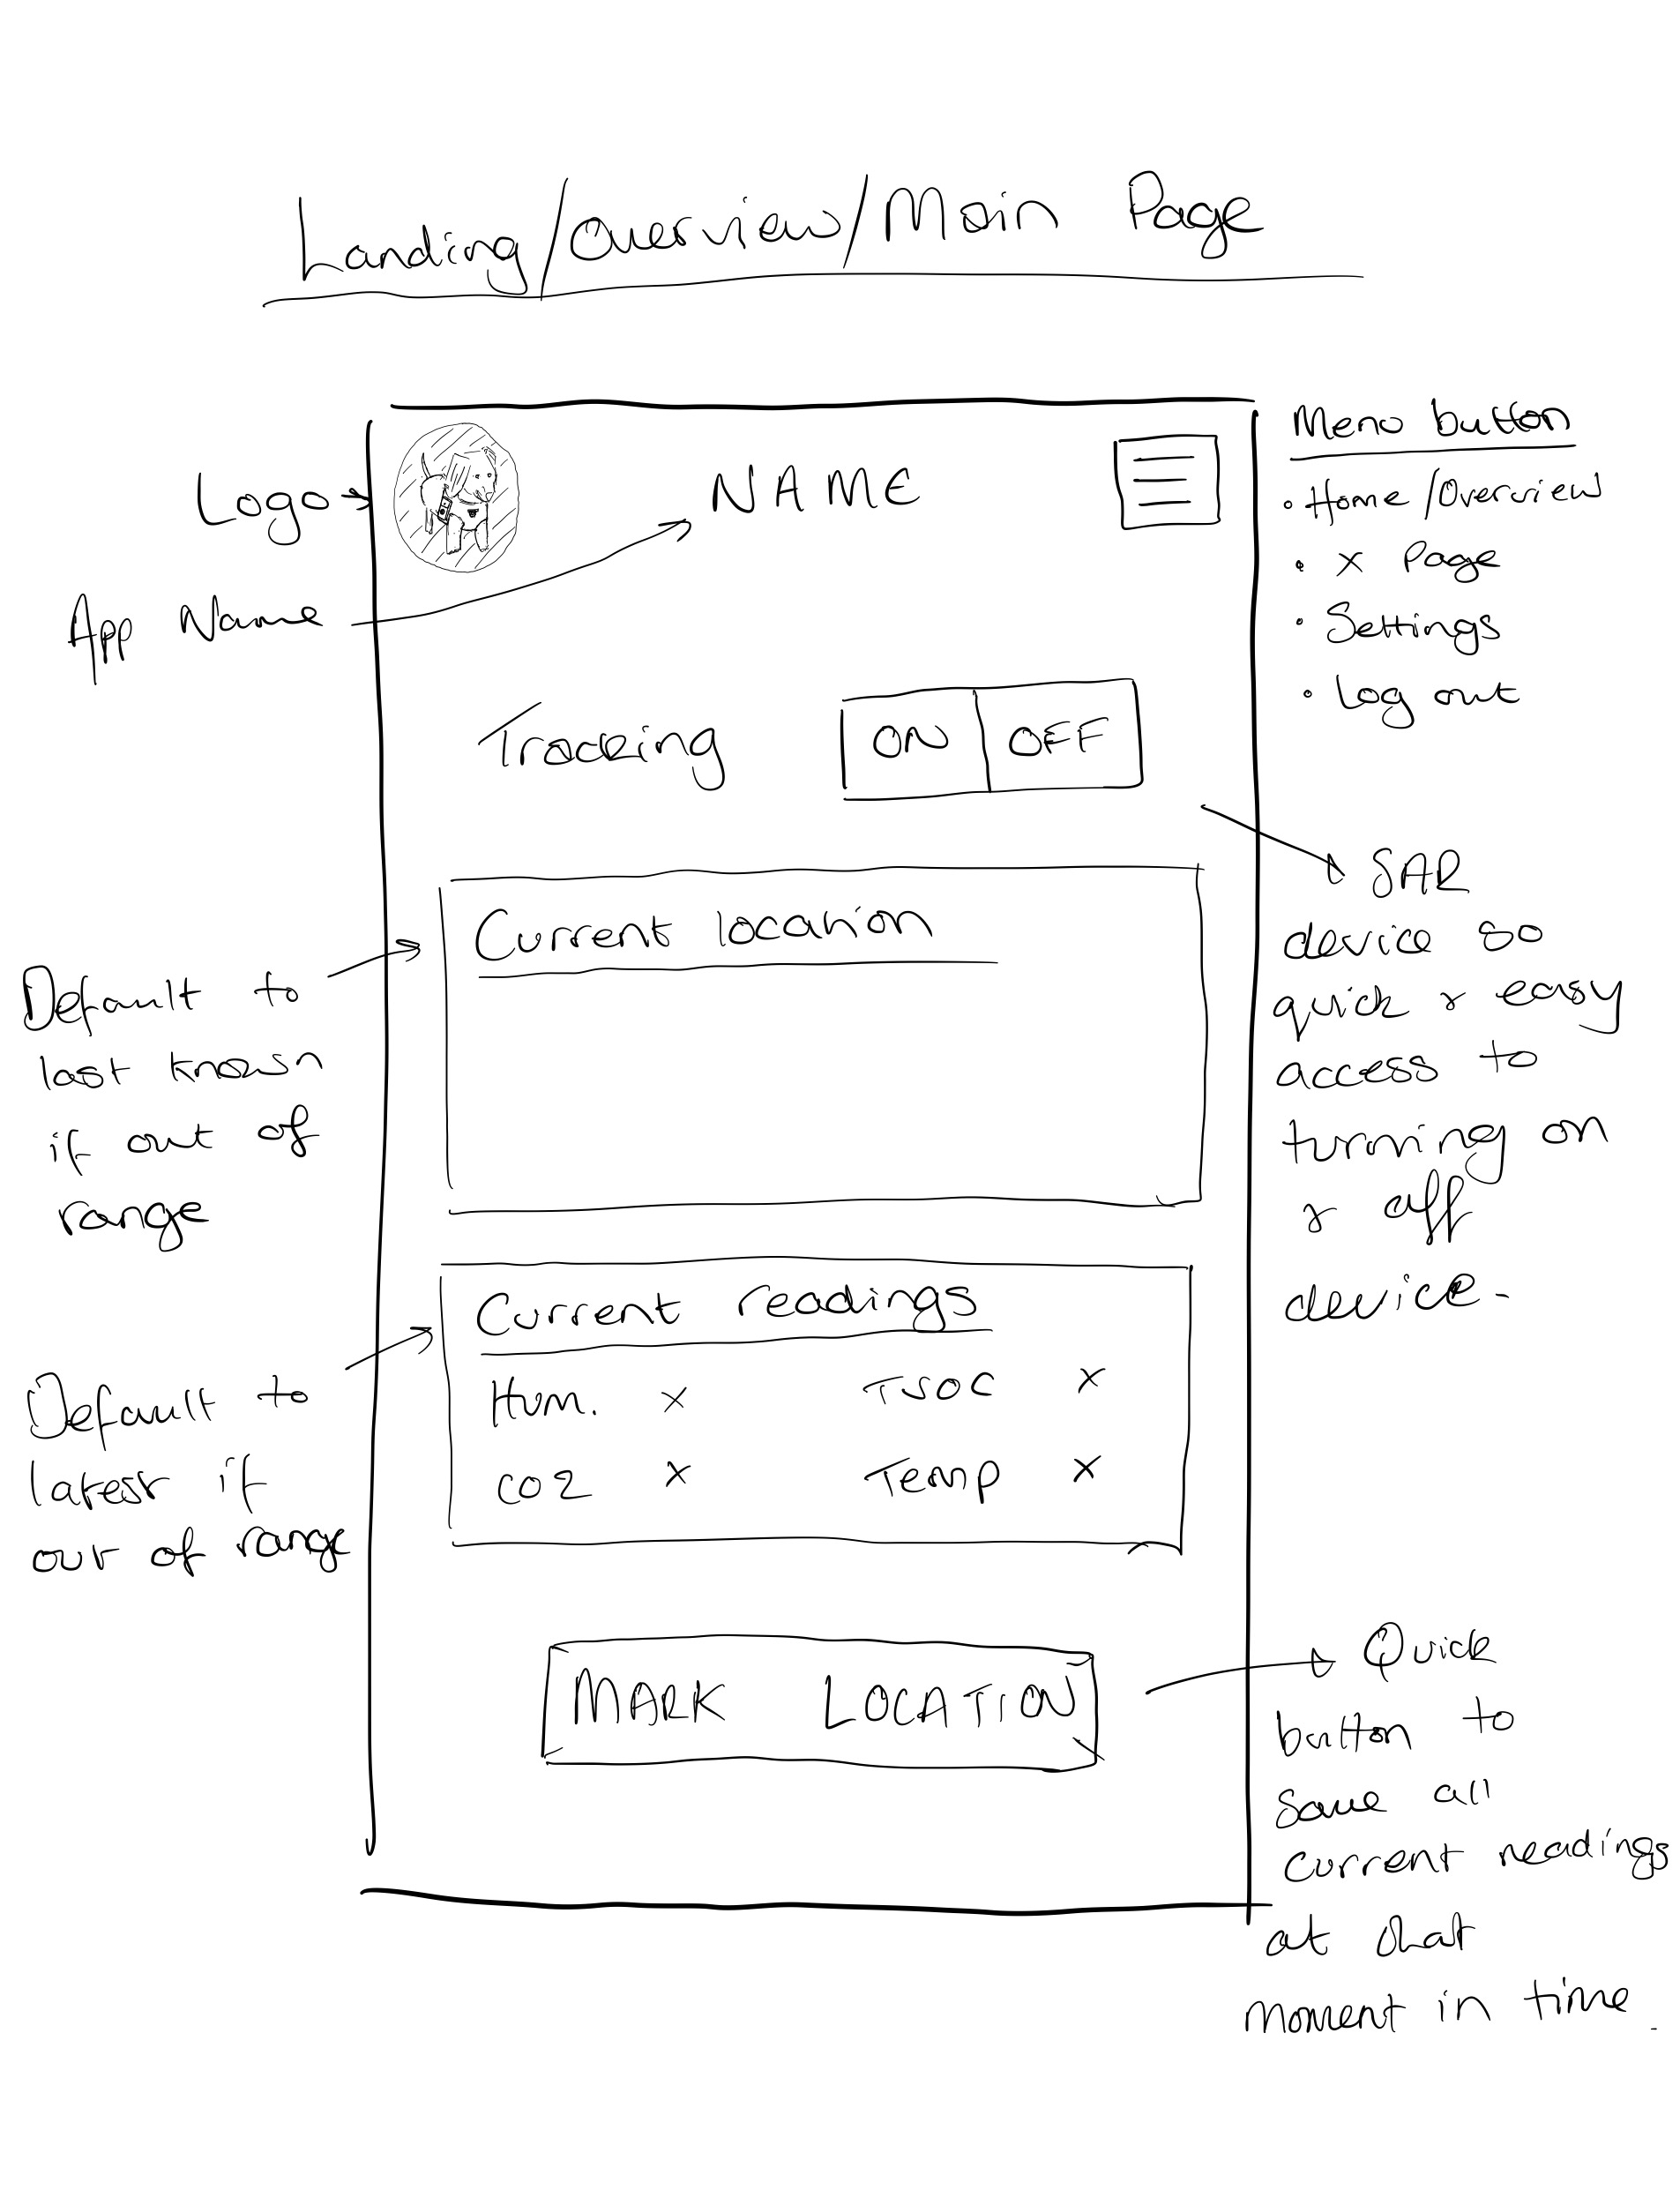
\includegraphics[width=\linewidth]{Images/Lofi_v1_c.jpg}
                \caption{Lo-Fi Prototype Version 1 Page 3}
                \label{Figure Lofi v1 3}
                
            \end{figure}
            \clearpage
            \begin{figure}[h]
                
                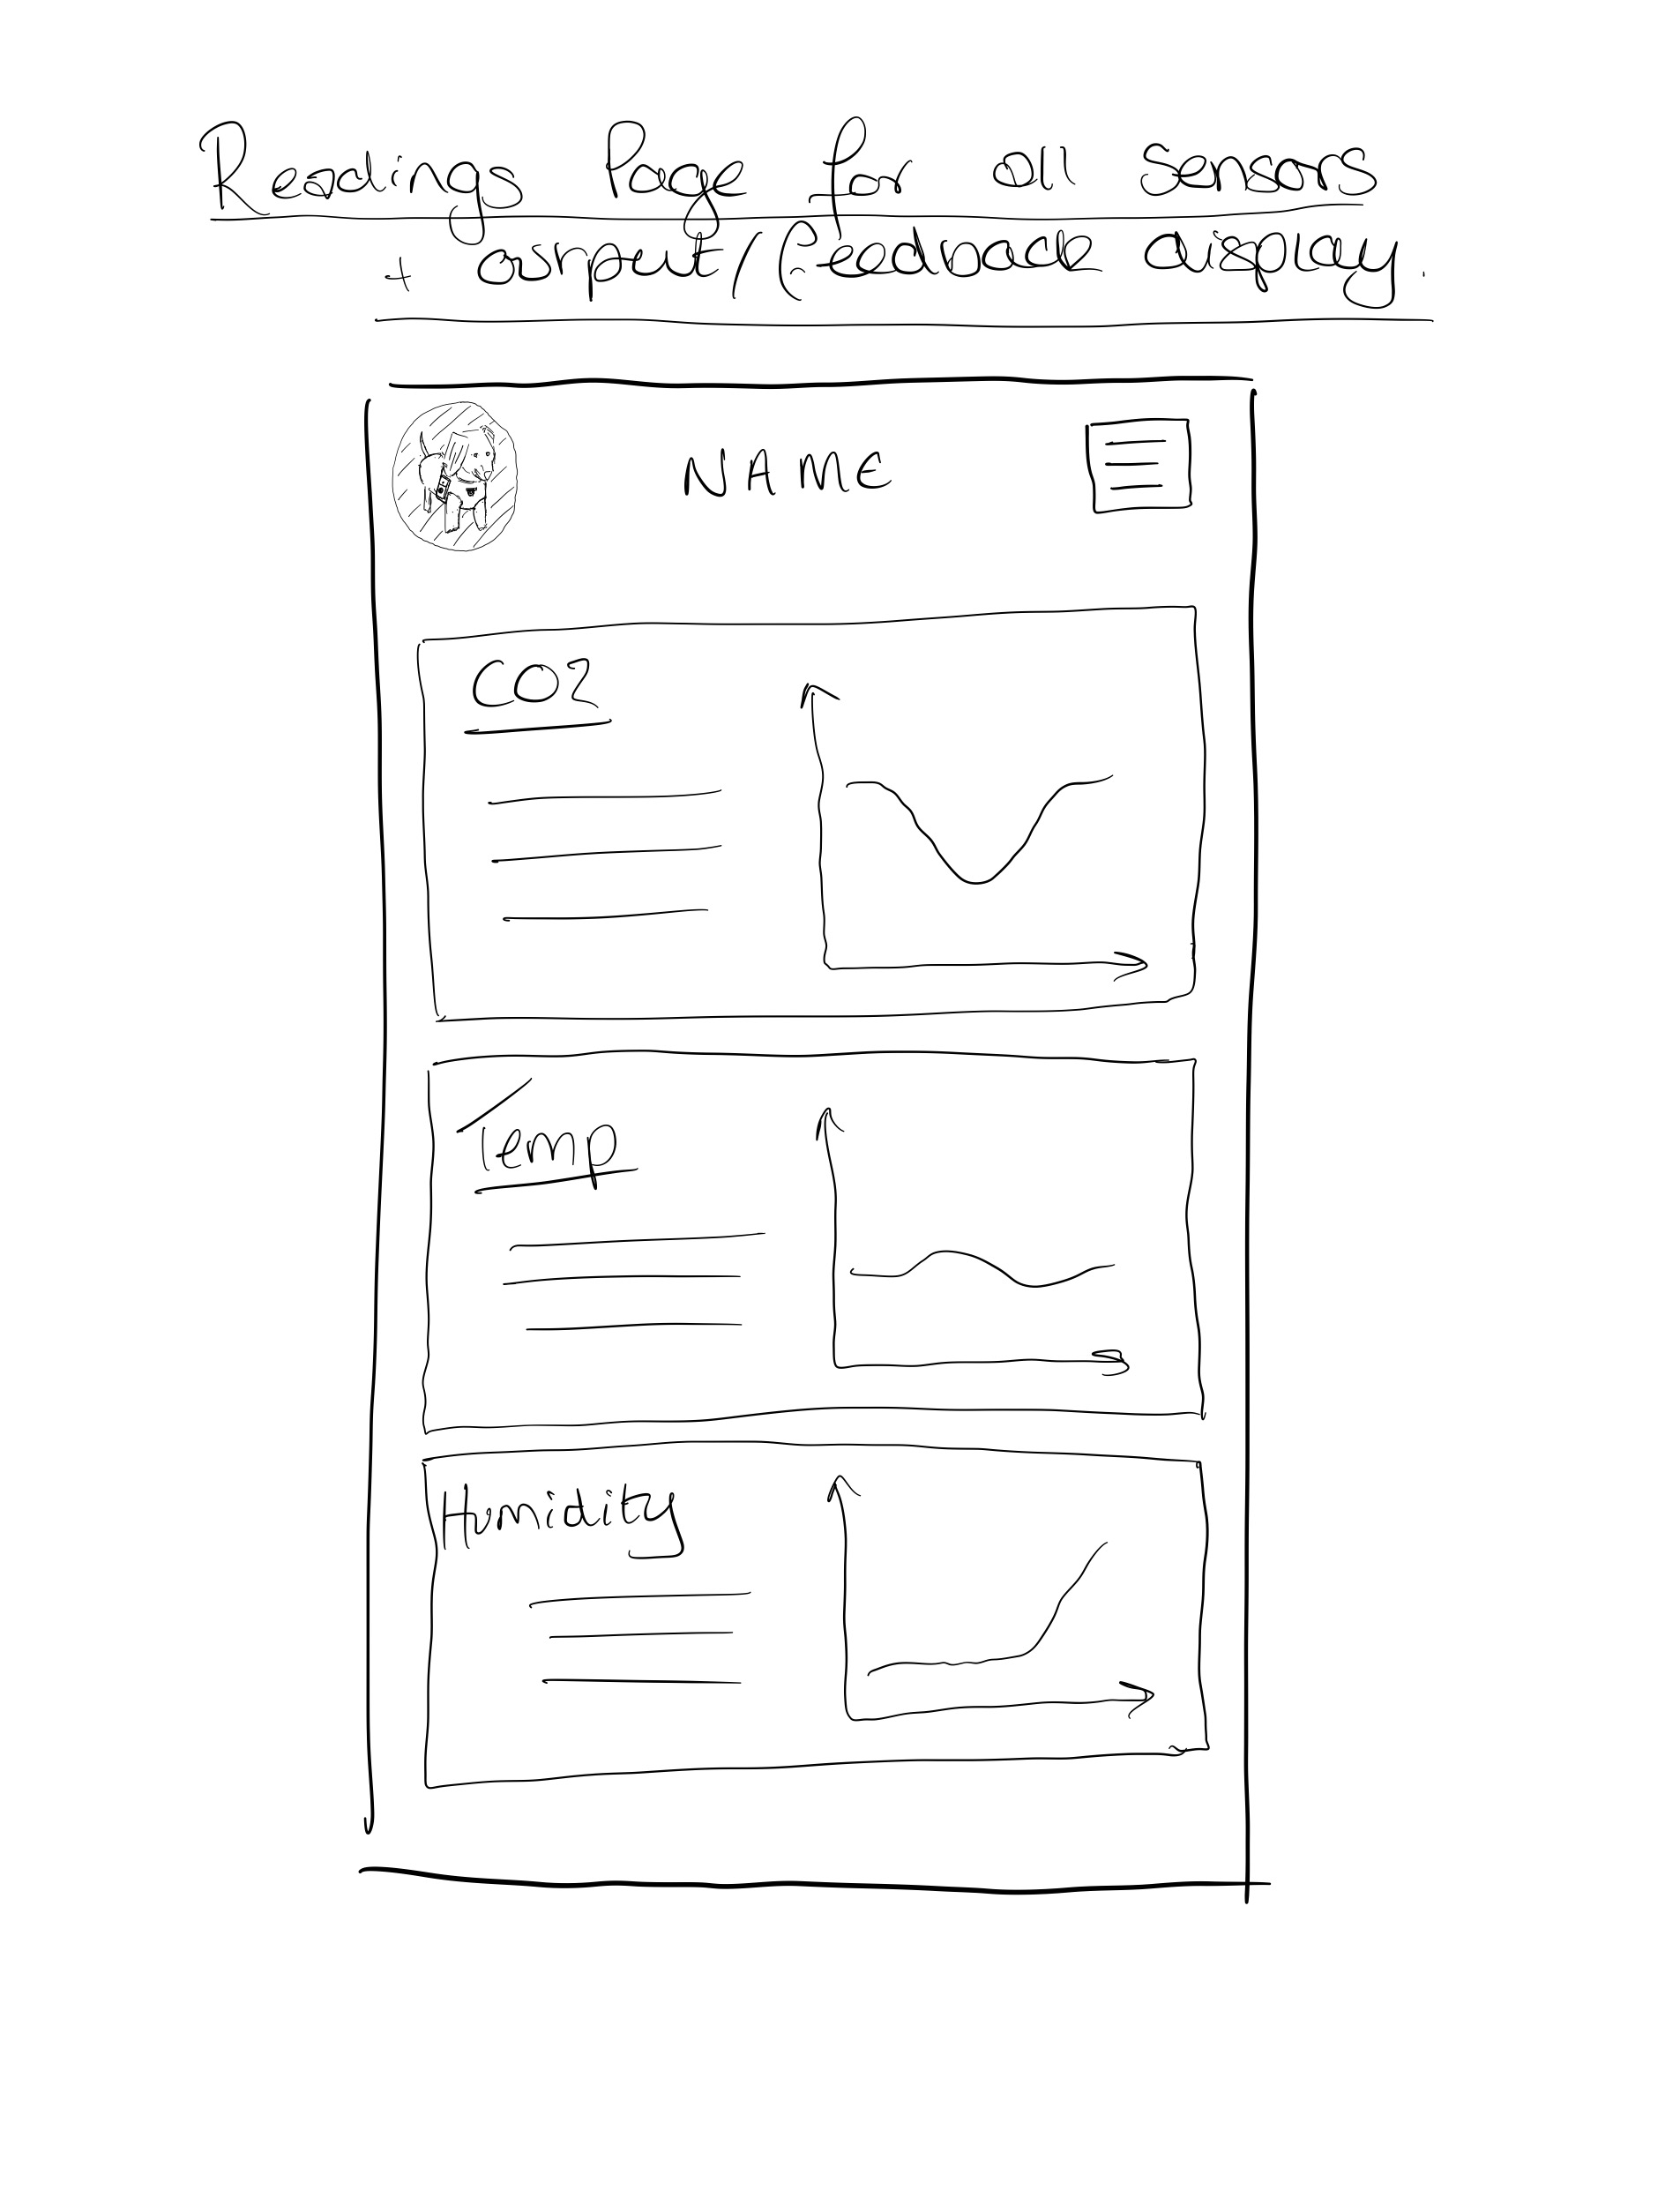
\includegraphics[width=\linewidth]{Images/Lofi_v1_d.jpg}
                \caption{Lo-Fi Prototype Version 1 Page 4}
                \label{Figure Lofi v1 4}
                
            \end{figure}
            \clearpage
            \begin{figure}[h]
                
                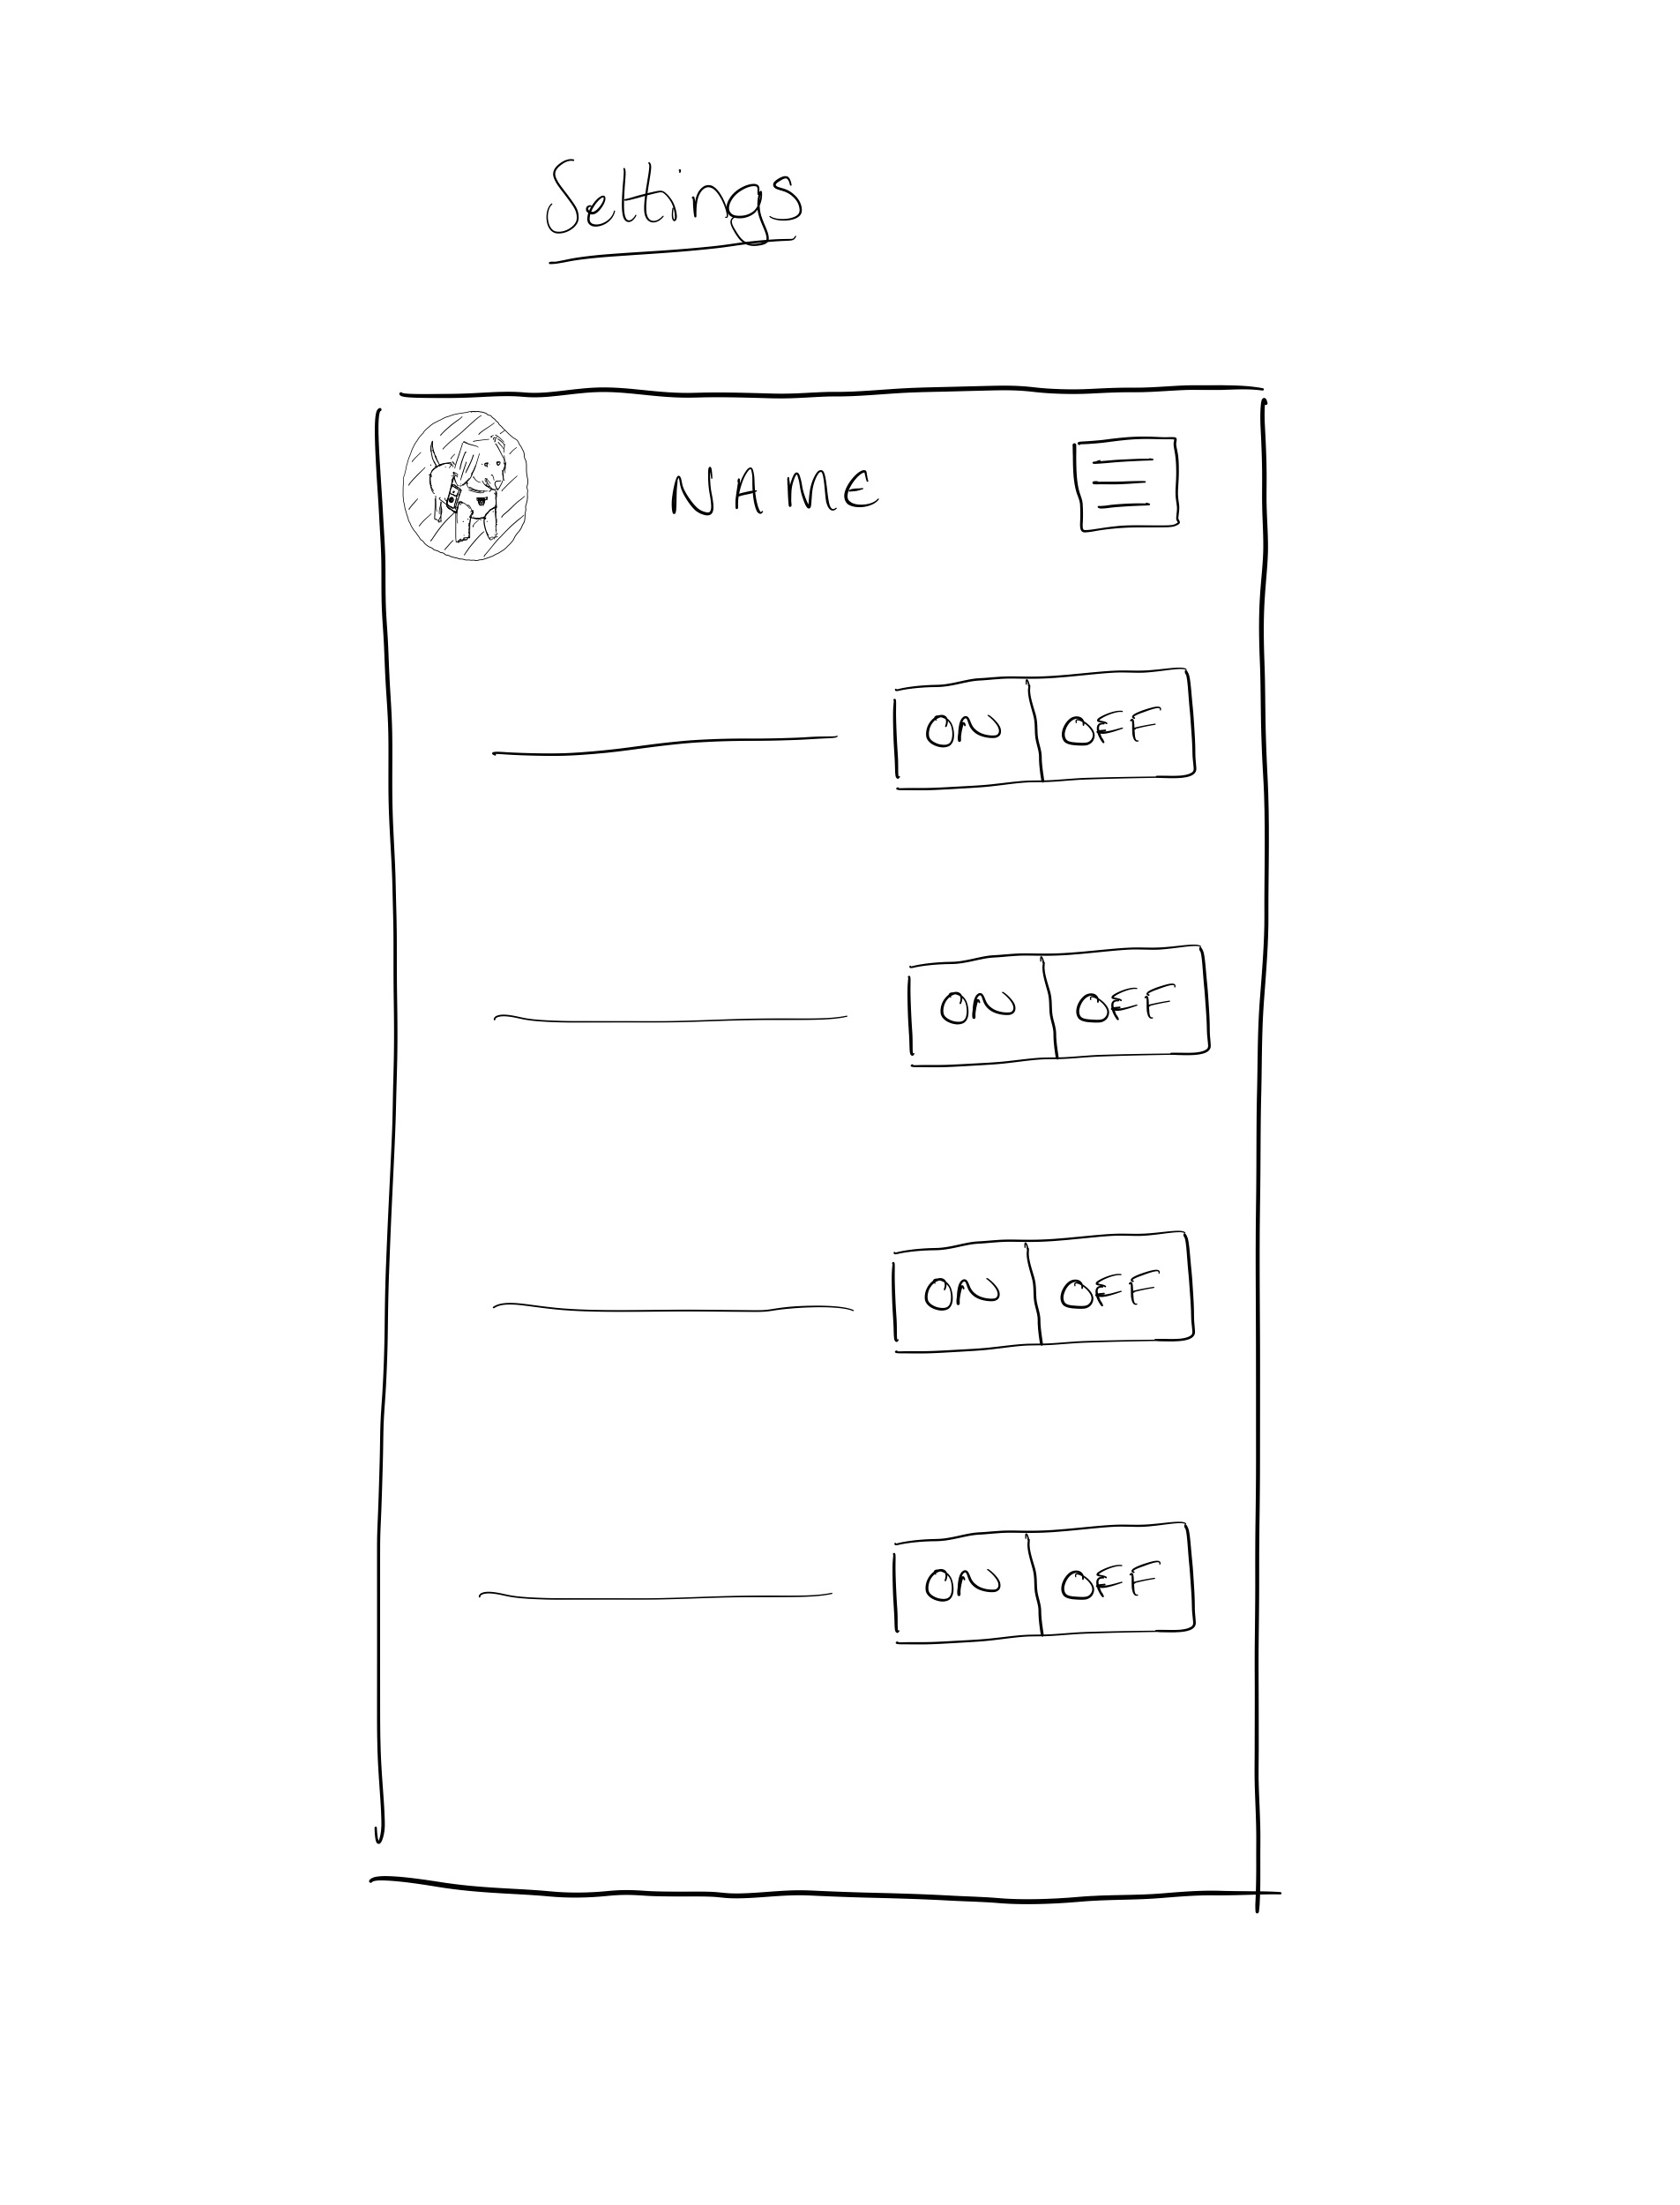
\includegraphics[width=\linewidth]{Images/Lofi_v1_e.jpg}
                \caption{Lo-Fi Prototype Version 1 Page 5}
                \label{Figure Lofi v1 5}
                
            \end{figure}
            \clearpage
            \begin{figure}[h]
                
                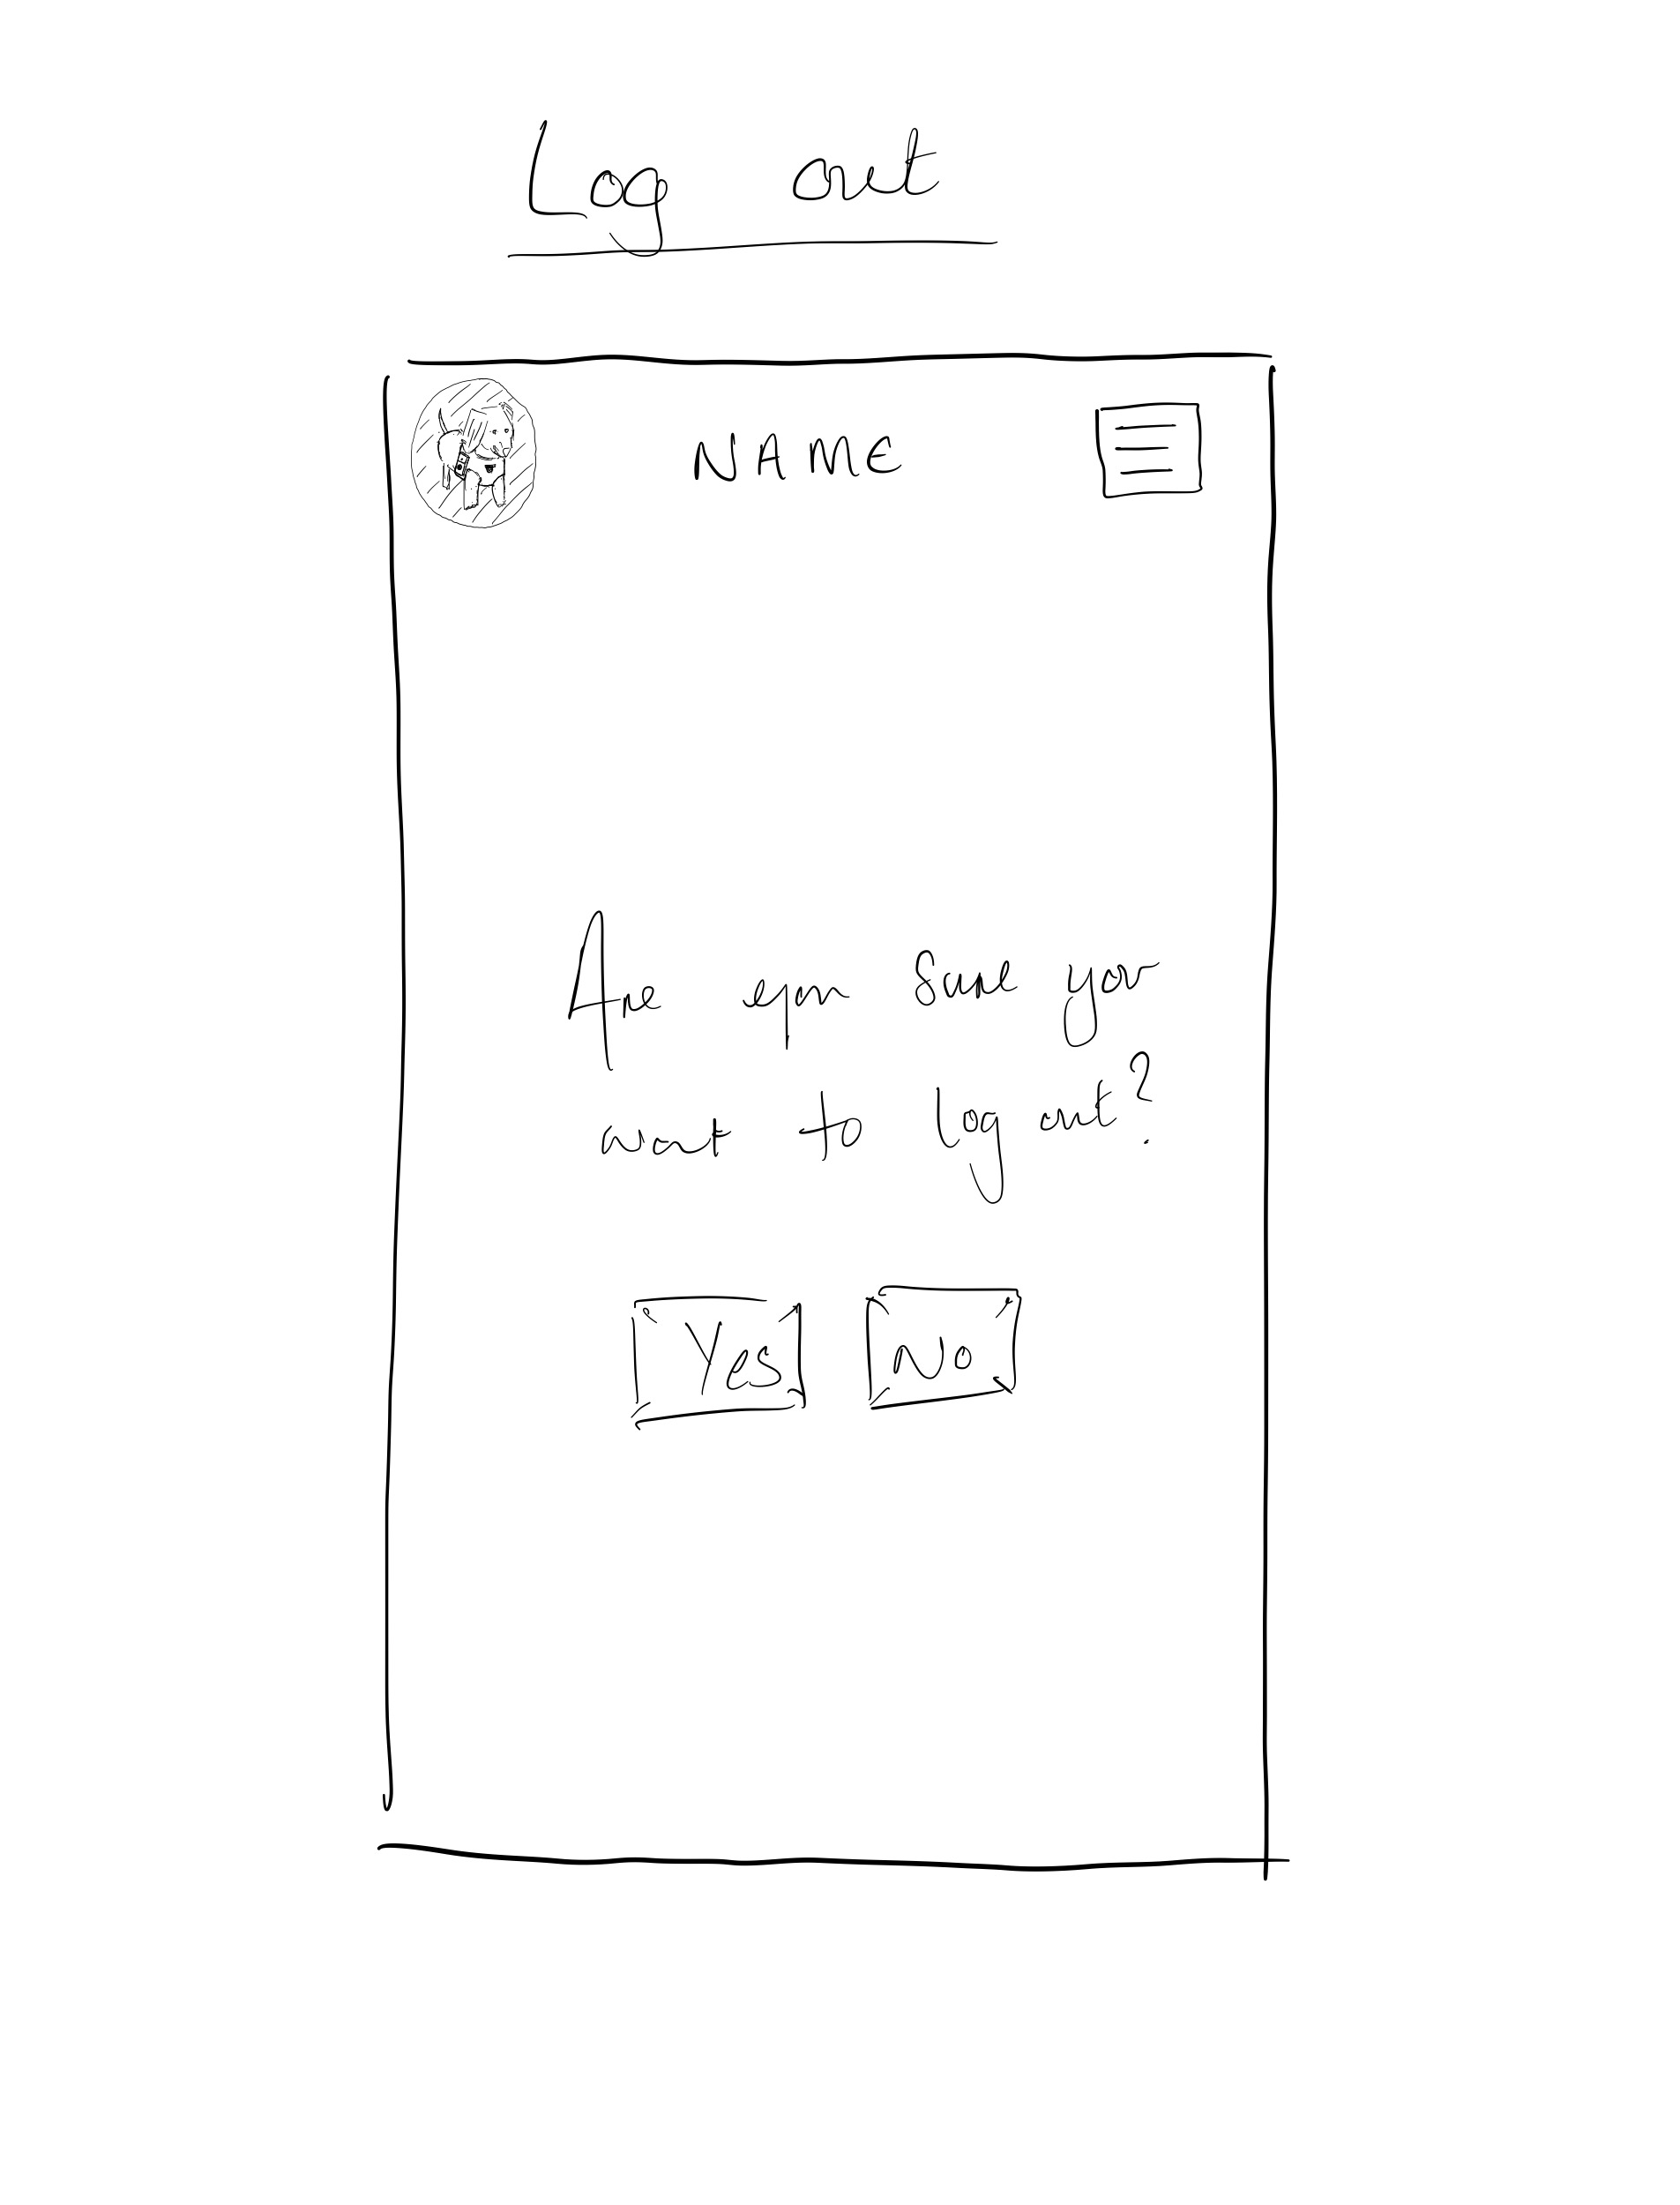
\includegraphics[width=\linewidth]{Images/Lofi_v1_f.jpg}
                \caption{Lo-Fi Prototype Version 1 Page 6}
                \label{Figure Lofi v1 6}
                
            \end{figure}
            \clearpage
            
            \subsection{Lo-Fi Prototypes Version 2}
            \begin{figure}[h]
                
                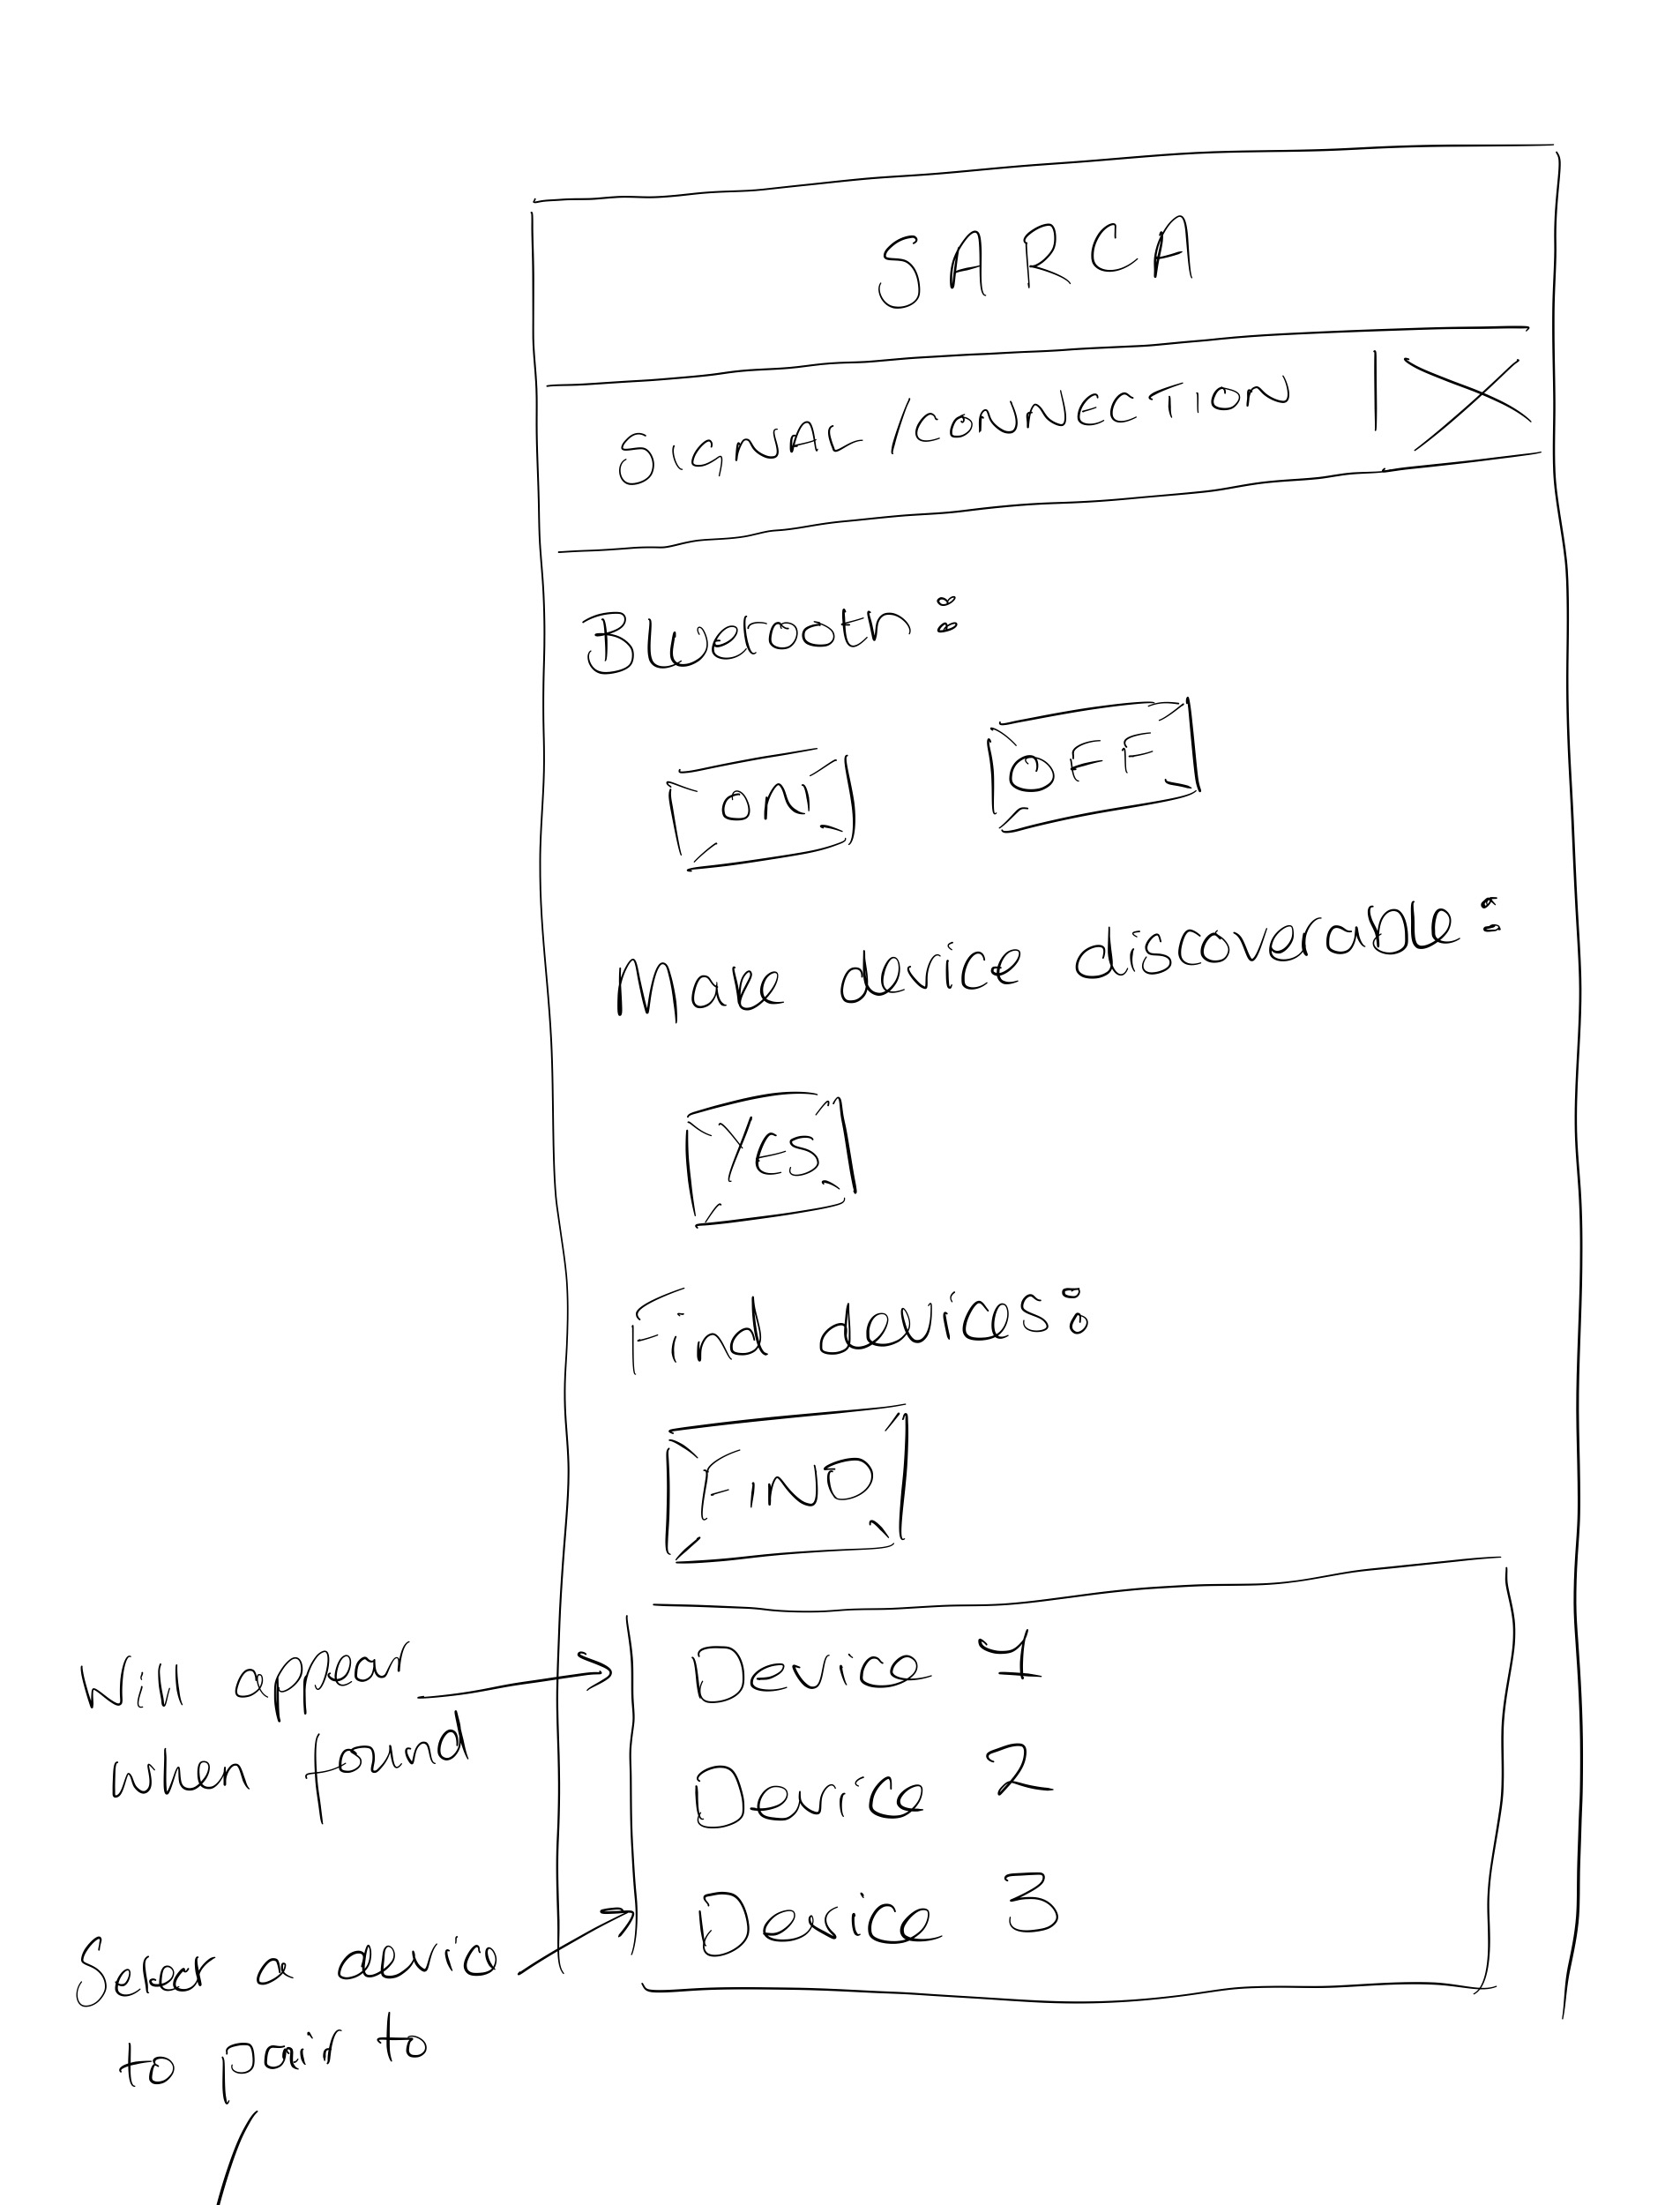
\includegraphics[width=\linewidth]{Images/Lofi_v2_a.jpg}
                \caption{Lo-Fi Prototype Version 2 Page 1}
                \label{Figure Lofi v2 1}
            
            \end{figure}
            \clearpage
            
            \begin{figure}[h]
                
                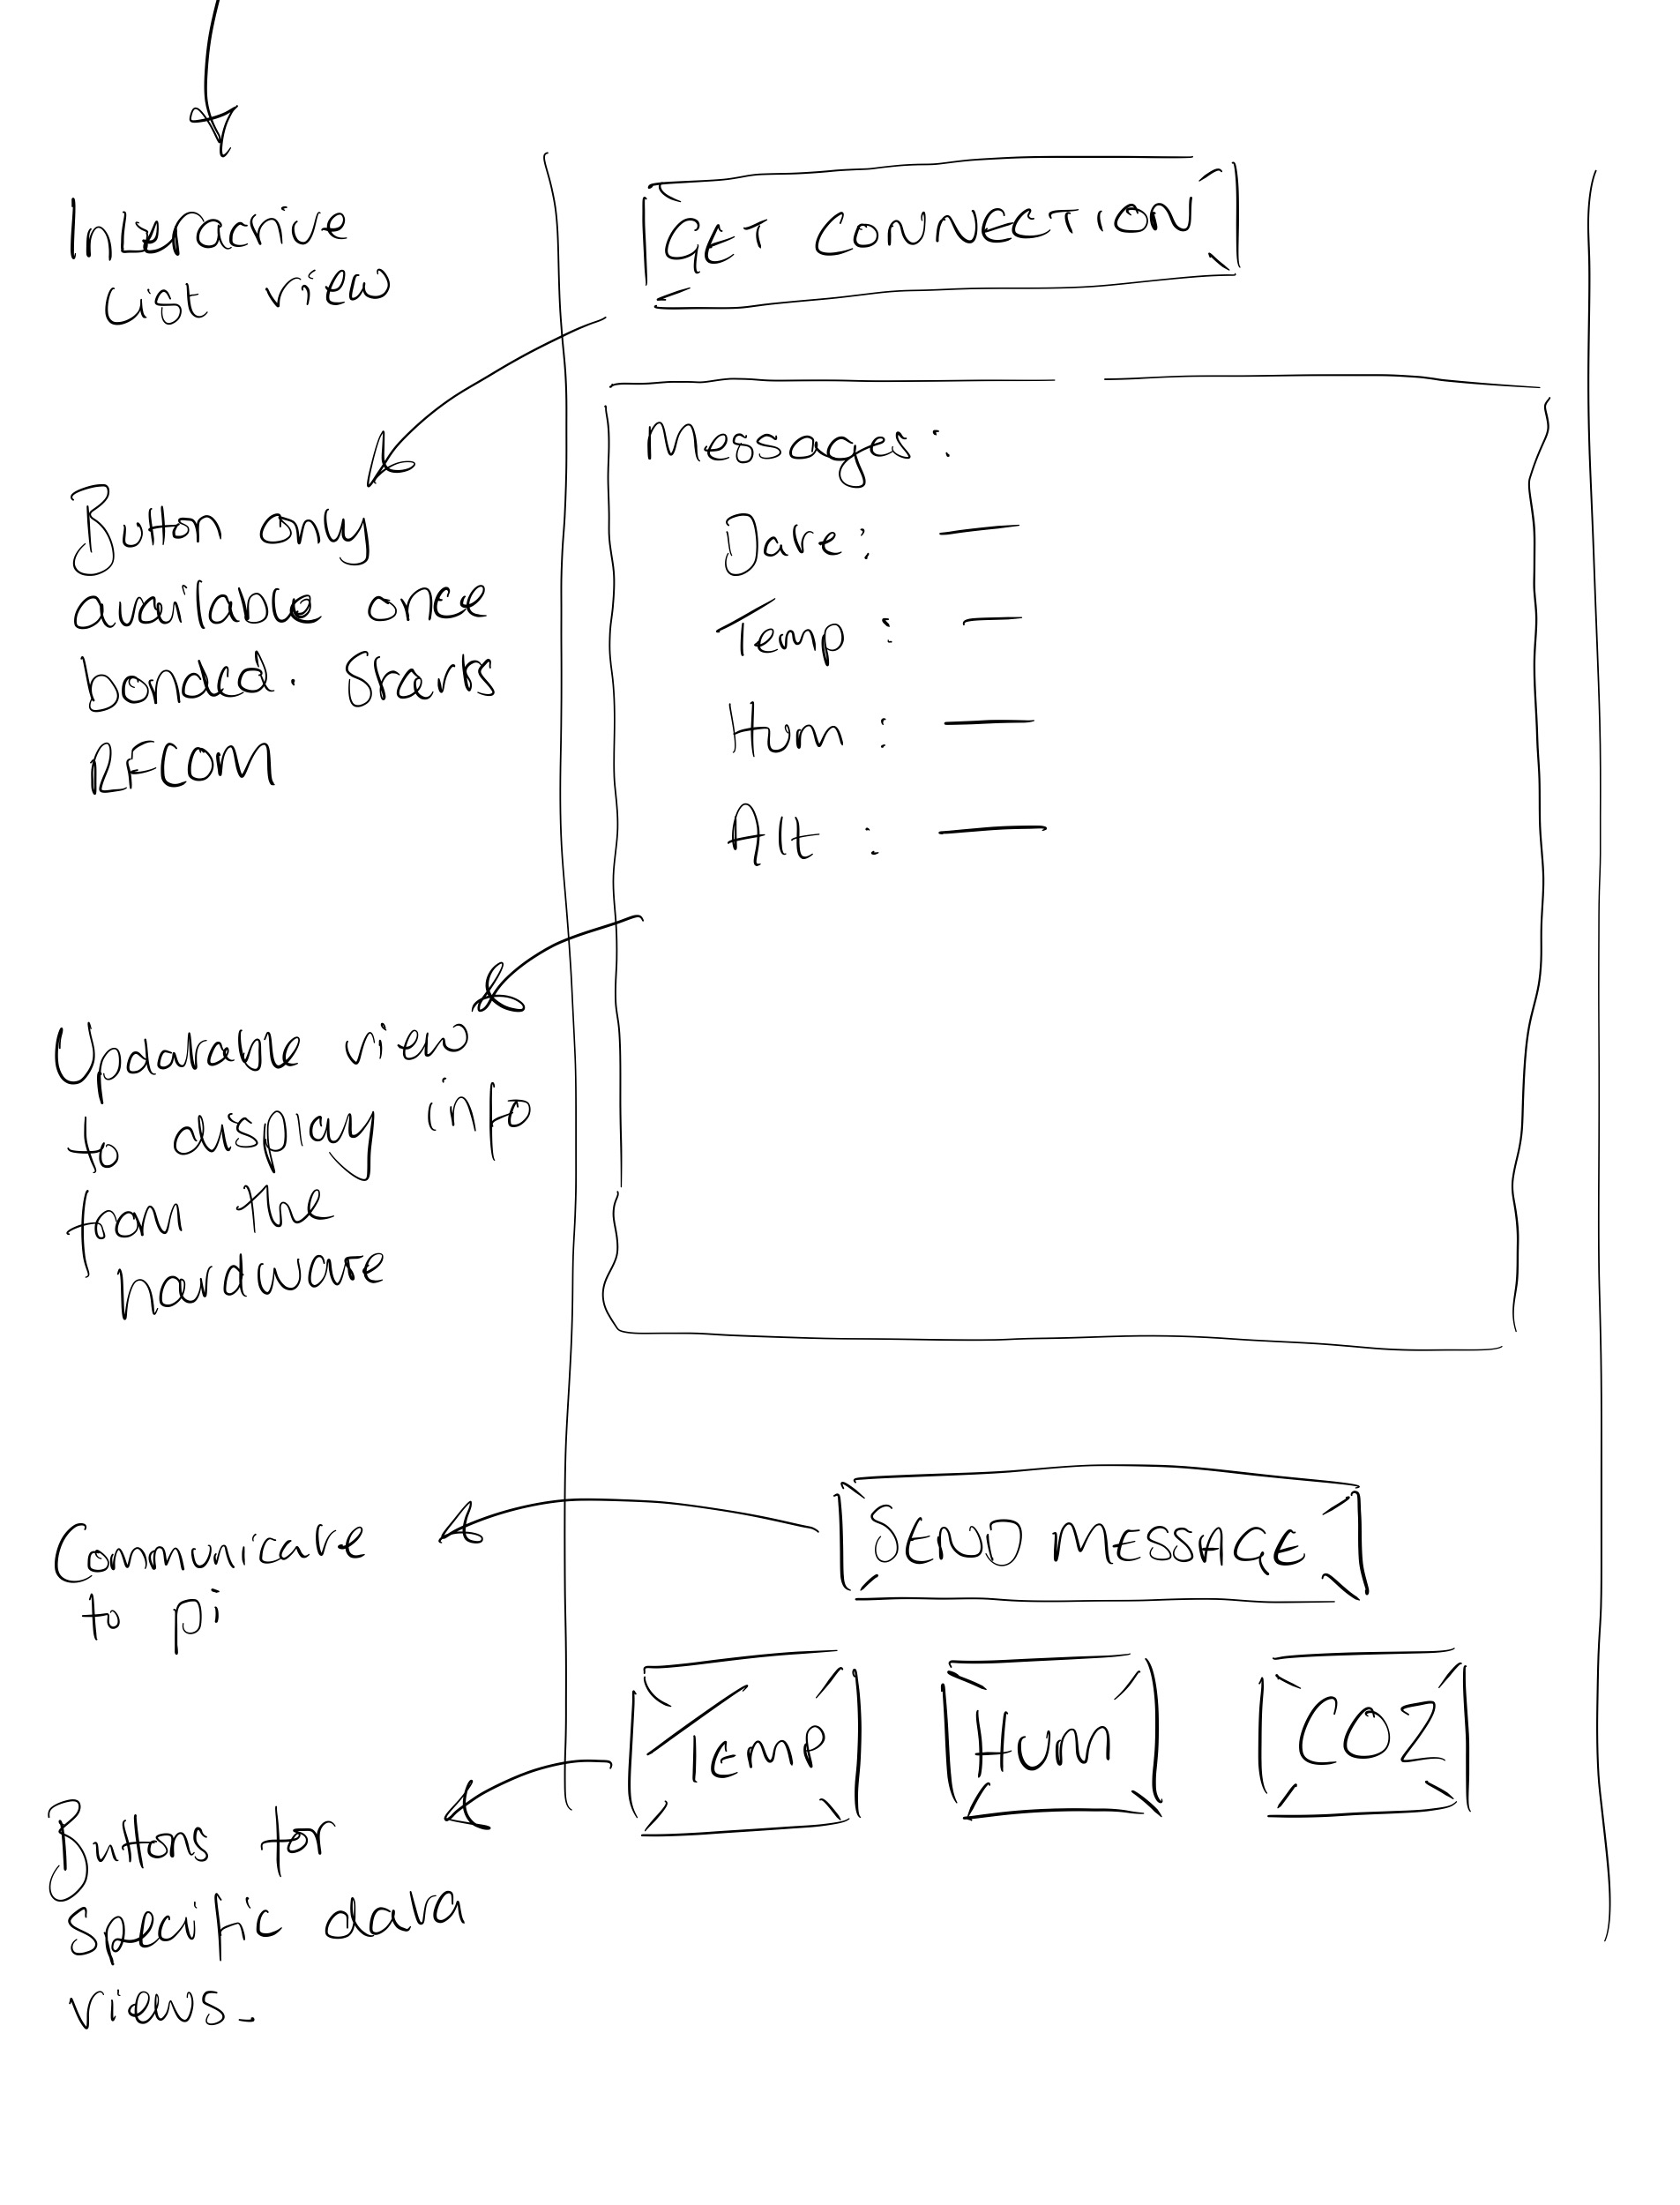
\includegraphics[width=\linewidth]{Images/Lofi_v2_b.jpg}
                \caption{Lo-Fi Prototype Version 2 Page 1}
                \label{Figure Lofi v2 2}
            
            \end{figure}
            \clearpage
            
        \section{Application}\label{app:application}
            \begin{figure}[h]
                \centering
                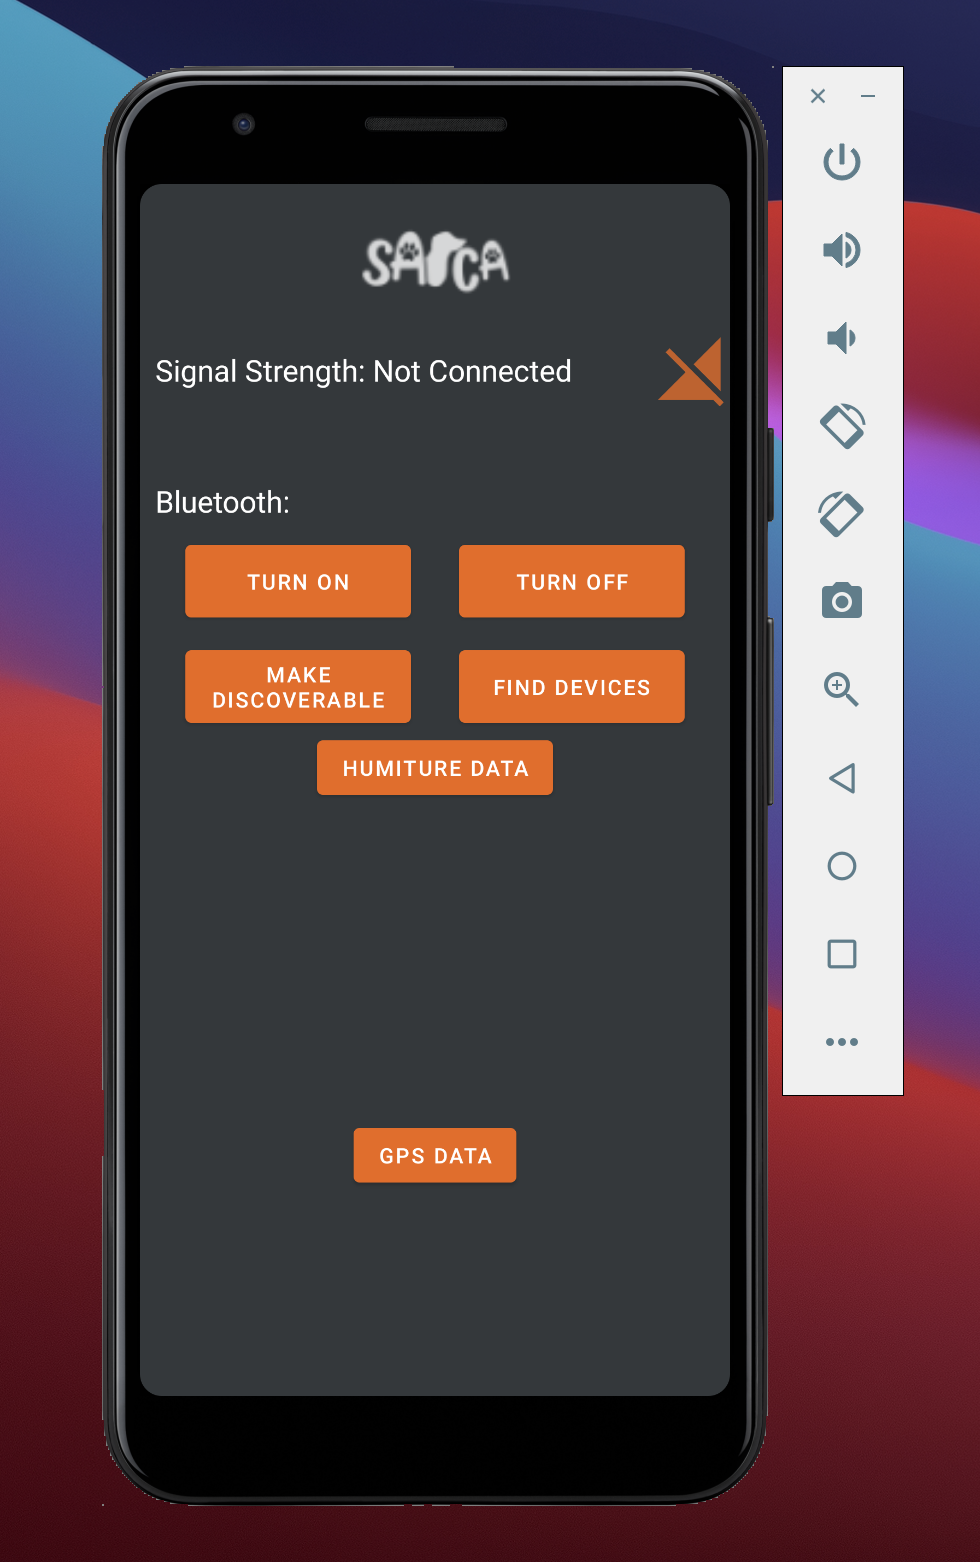
\includegraphics[scale=0.75]{Images/App_photo_1.png}
                \caption{Application Screenshot Before Connection}
                \label{Figure App before connection}
            
            \end{figure}
            \clearpage
            
            \begin{figure}[h]
                \centering
                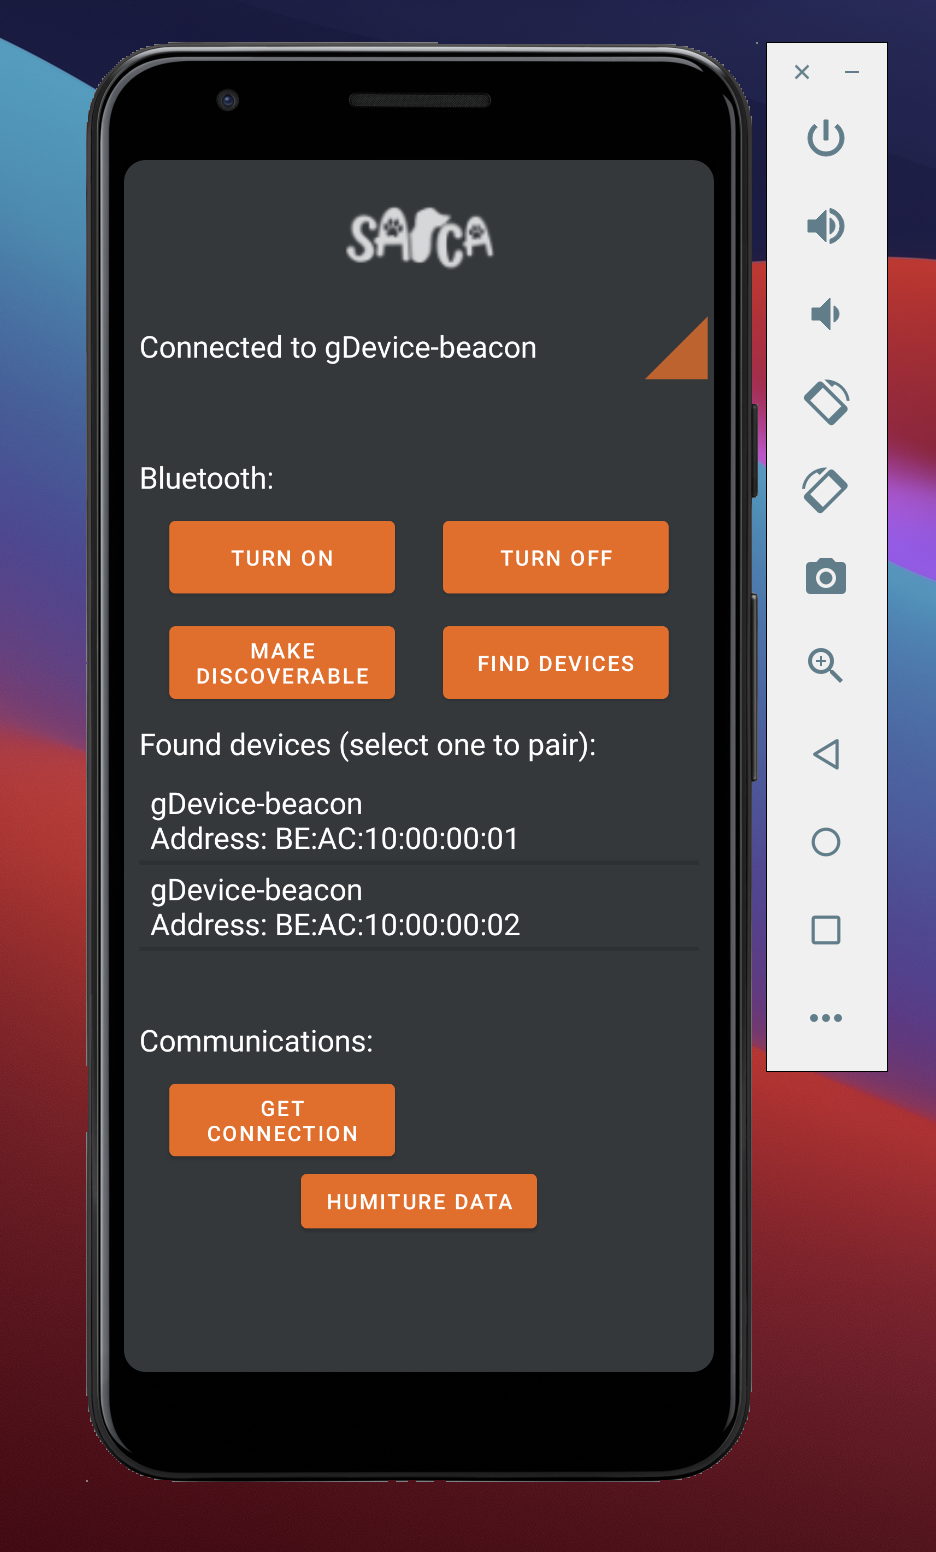
\includegraphics[scale=0.75]{Images/App_photo_2.png}
                \caption{Application Screenshot Bond Established}
                \label{Figure App Bonded}
            
            \end{figure}
            \clearpage
            
            \begin{figure}[h]
                \centering
                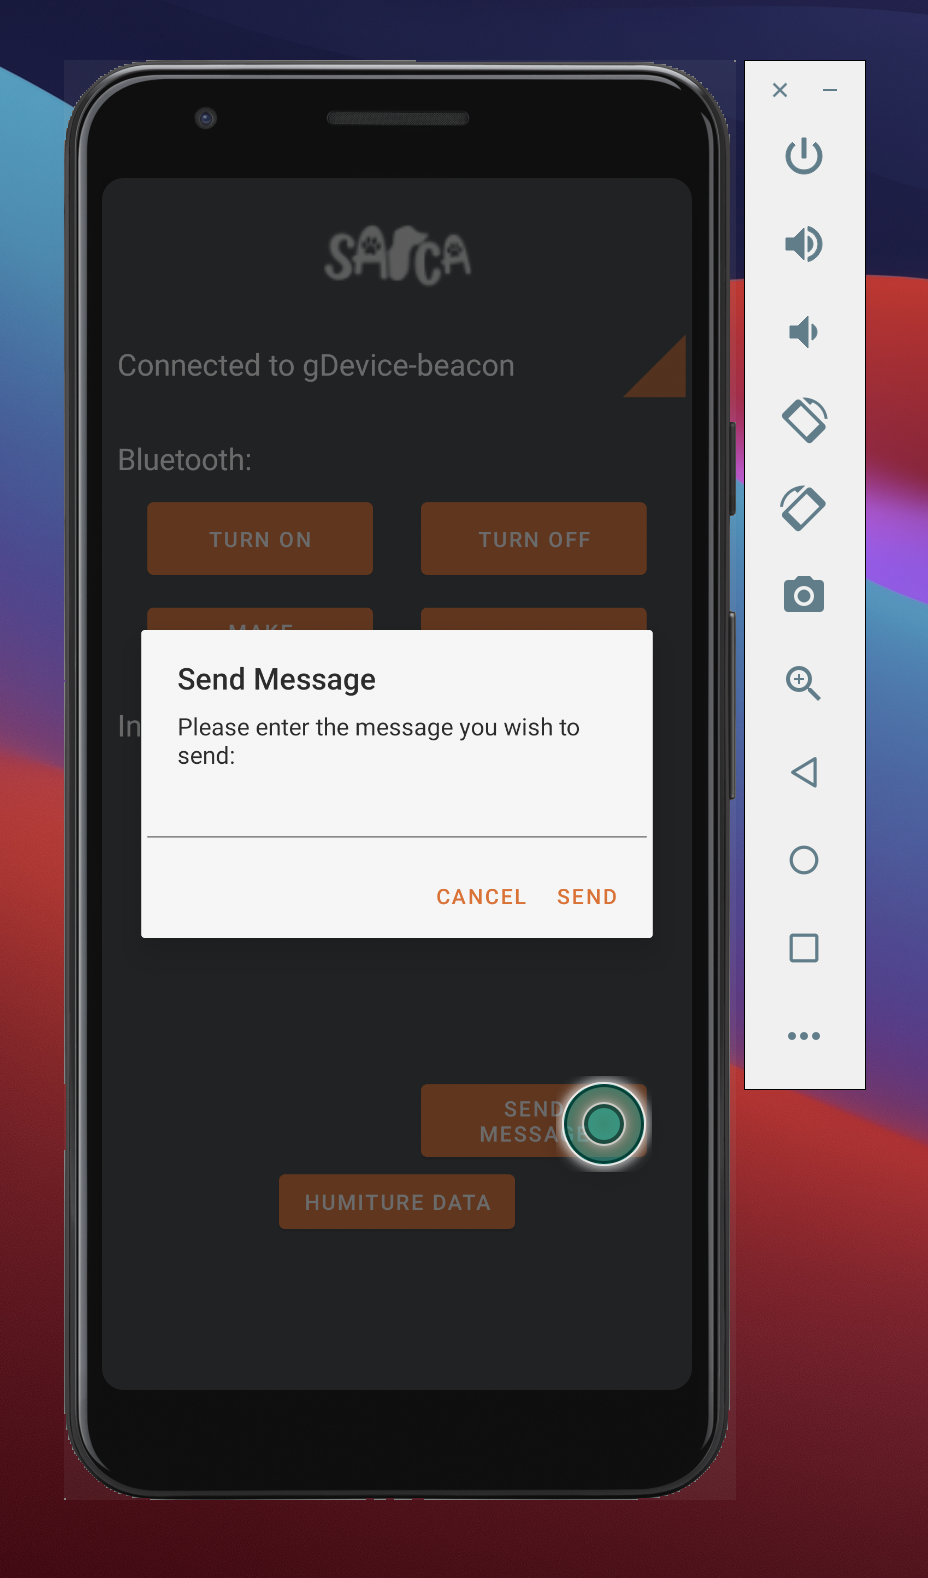
\includegraphics[scale=0.75]{Images/App_photo_3.png}
                \caption{Application Screenshot Send Message}
                \label{Figure App Send Message}
            
            \end{figure}
            \clearpage
            \begin{figure}[h]
                \centering
                \includegraphics[width=\linewidth]{Images/main.png}
                \caption{Application In Action}
                \label{Figure App In Action}
            
            \end{figure}
            \clearpage
            
            \begin{figure}[h]
                \centering
                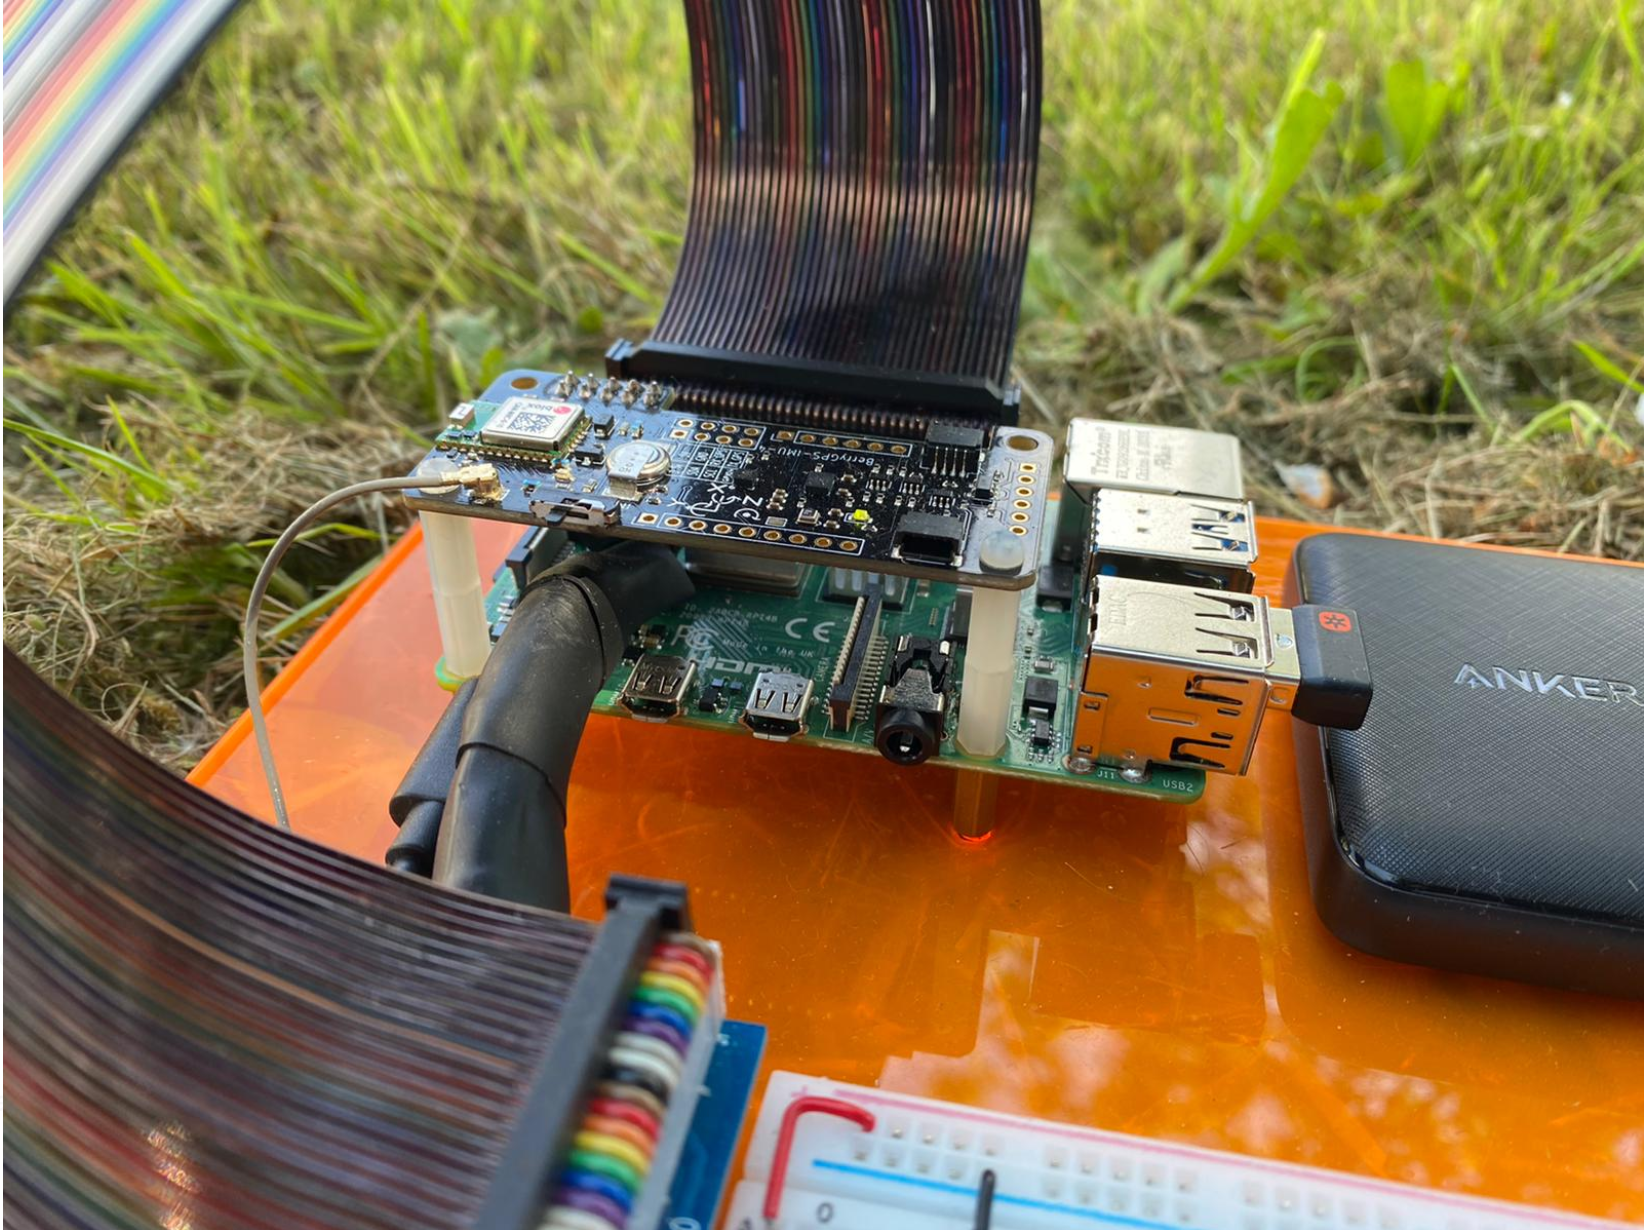
\includegraphics[width=\linewidth]{Images/berry.png}
                \caption{Application In Action}
                \label{Figure App In Action}
            
            \end{figure}
            \clearpage
            \begin{figure}[h]
                \centering
                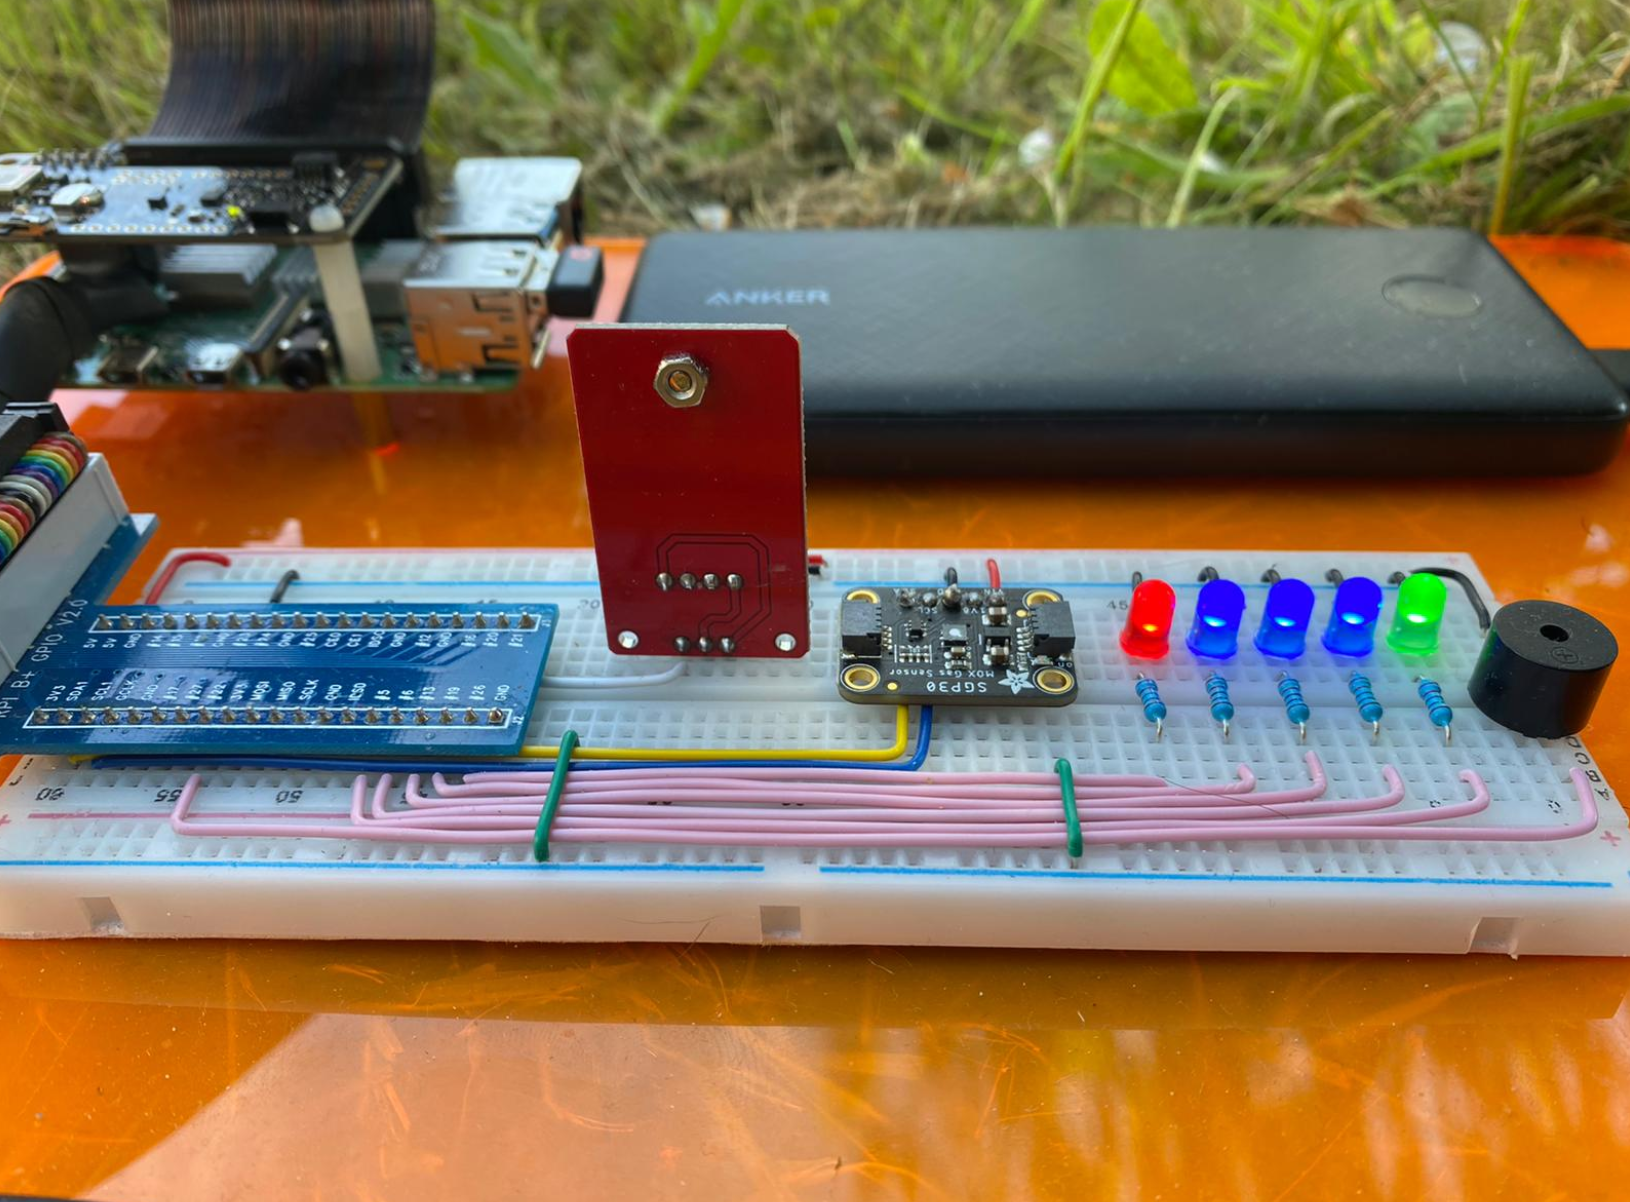
\includegraphics[width=\linewidth]{Images/bread.png}
                \caption{Application In Action}
                \label{Figure App In Action}
            
            \end{figure}
            \clearpage
            \begin{figure}[h]
                \centering
                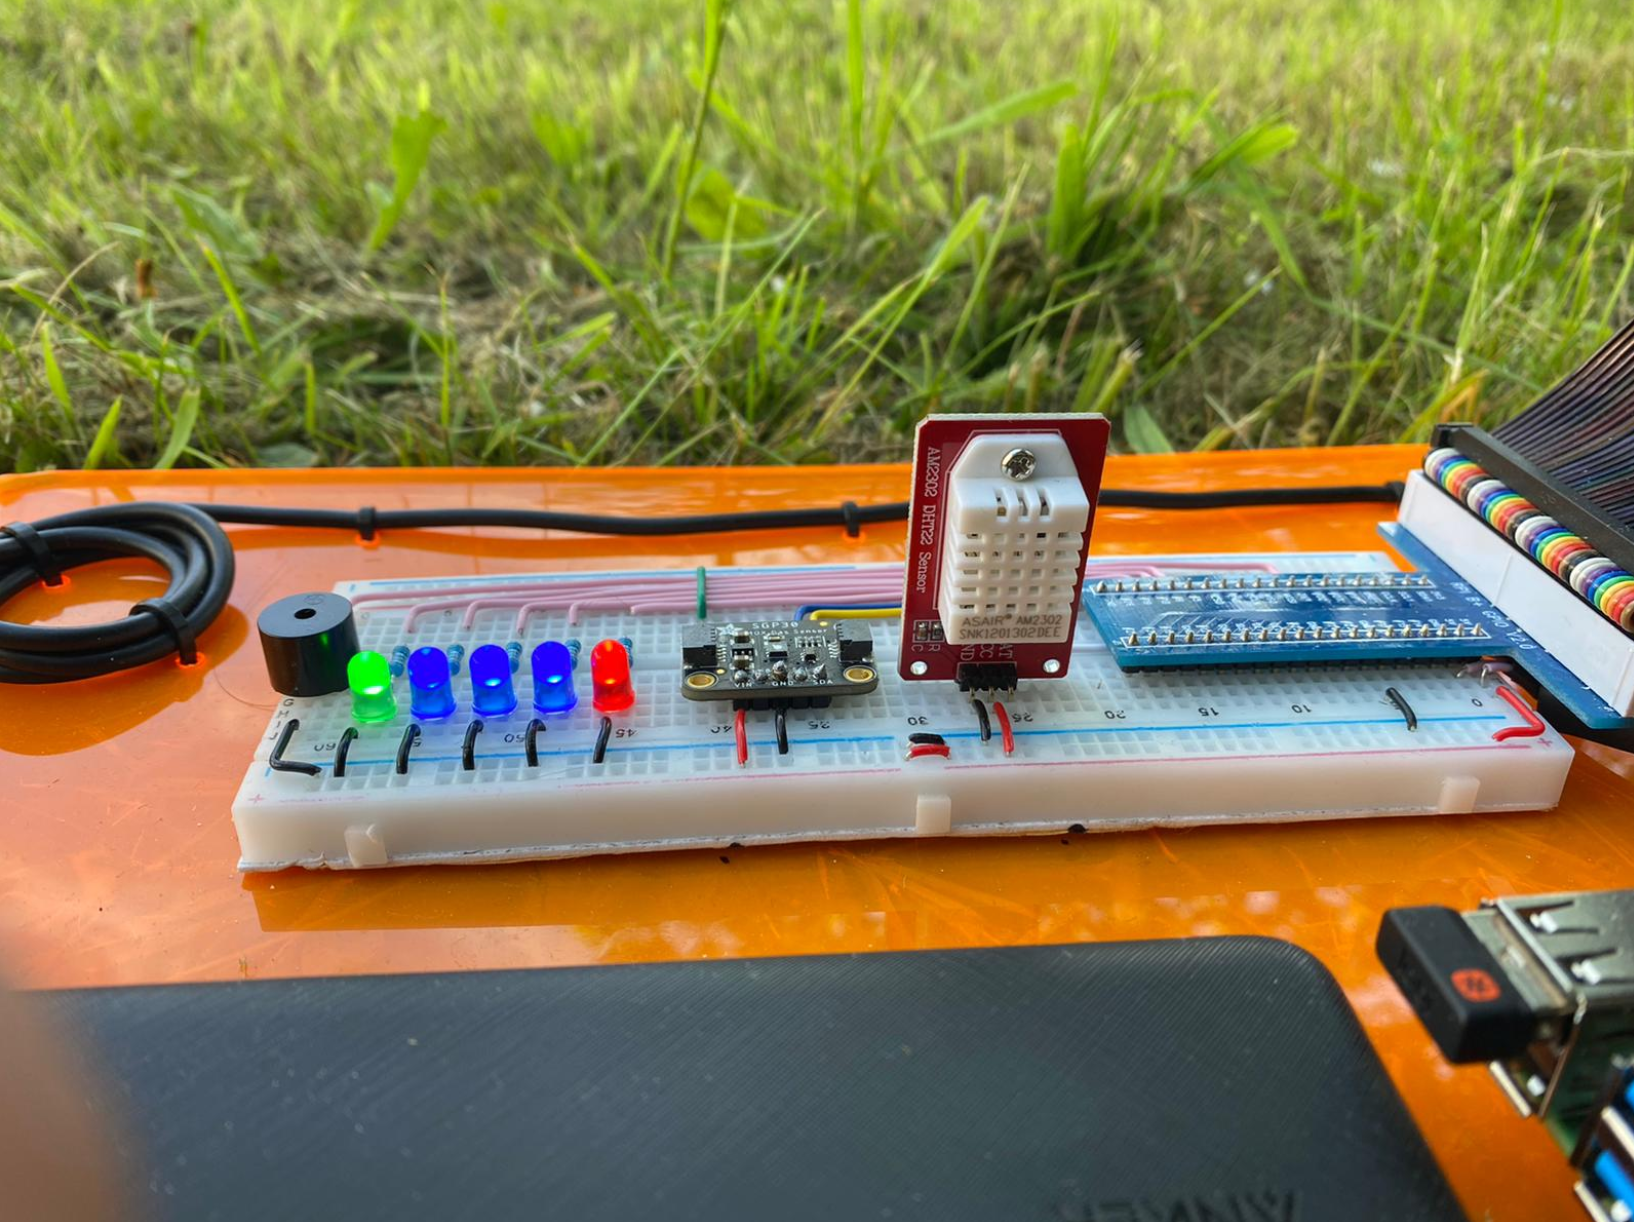
\includegraphics[width=\linewidth]{Images/bread2.png}
                \caption{Application In Action}
                \label{Figure App In Action}
            
            \end{figure}
            \clearpage
        

\end{document}
